\chapter{Portfolio Optimization}
\label{portfolio-optimization}

Portfolio optimization models look for the optimal way to make investments. Usually investors expect either a maximum return for a given level of risk or a given return for a minimum risk so these models are typically based on two criteria: maximization of the expected return and/or minimization of the risk.

While the concept of return is straightforward there are a variety of risk measures. The most popular one is the variance in return and we will mainly focus on it in this Chapter.

Some notations that will be used later are

\begin{itemize}
\tightlist
\item
  portfolio expected return: 
  \begin{equation} 
  	\mathbb{E}(R_{p}) = \sum _{i}w_{i} \mathbb{E}(R_{i}) = \mathbf{w}\cdot \mathbb{E}(\mathbf{R}) = \mathbf{w}^T \mathbb{E}(\mathbf{R})=
      \begin{bmatrix}
      w_1 \\ 
      w_2 \\ 
      \vdots \\
      w_n
      \end{bmatrix}
      \begin{bmatrix}
      \mathbb{E}(R_1) & \mathbb{E}(R_2) & \cdots & \mathbb{E}(R_n)
      \end{bmatrix}
  \end{equation} 
  where \(R_{p}\) is the return on the portfolio, \(R_{i}\) is the return on asset \(i\) and \(w_{i}\) is the weighting of component asset \(i\) (that is, the proportion of asset \(i\) in the portfolio) and \(\sum_{i}w_i = 1\) and \(0 \le w_i \le 1\);
\item
  portfolio return variance:
  \begin{equation}
  \begin{aligned}
  \sigma _{p}^{2} = &\sum _{i}\sum _{j}w_{i}w_{j}\sigma _{ij} = \mathbf{w}^T\Sigma\mathbf{w} =
  \begin{bmatrix}
  w_1 \\ 
  w_2 \\ 
  \vdots \\
  w_n
  \end{bmatrix}
  \begin{bmatrix}
  \sigma_{11} & \sigma_{12} & \cdots & \sigma_{1n} \\
  \sigma_{21} & \sigma_{22} & \cdots & \sigma_{2n} \\
  \vdots & & \\
  \sigma_{n1} & \sigma_{n2} & \cdots & \sigma_{nn} \\
  \end{bmatrix}
  \begin{bmatrix}
  w_1 & w_2 & \cdots & w_n
  \end{bmatrix} =\\ 
  &\begin{bmatrix}
  \sigma_{11} *w_1 + \sigma_{12} *w_2 + \cdots + \sigma_{1n}*w_n \\
  \sigma_{21} *w_1 + \sigma_{22} *w_2  +\cdots + \sigma_{2n}*w_n \\
  \vdots \\
  \sigma_{n1} *w_1 + \sigma_{n2}*w_2 + \cdots + \sigma_{nn}*w_n \\
  \end{bmatrix}
  \begin{bmatrix}
  w_1 & w_2 & \cdots & w_n
  \end{bmatrix}
  \end{aligned}
  \end{equation}
  where \(\sigma\) is the (sample) standard deviation of the periodic returns on an asset, and \(\rho _{ij}\) is the correlation coefficient between the returns on assets \(i\) and \(j\). For a brief introduction to matrices see Chapter~\ref{sec:matrices};
\item
  portfolio return volatility (standard deviation):
  \begin{equation}
  	\sigma _{p}= \sqrt{\sigma _{p}^{2}}
  \end{equation}
\end{itemize}

\section{Modern Portfolio Theory}
\label{the-markowitz-meanvariance-portfolio-model}

Although investors may expect a particular return when buying a stock, they also may be disappointed or pleasantly surprised, because fluctuations in stock prices result in fluctuating returns. 

The Modern Portfolio Theory (MPT), introduced by Markowitz, defines risk as the possibility that actual returns will deviate from expected returns (the degree of potential fluctuation determines the degree of risk).
So it assumes that an investor has two considerations when constructing an investment portfolio: expected return and variance in return (i.e. measure of risk). 

Hence the Markowitz model requires two major information:

\begin{itemize}
\tightlist
\item the estimated expected return for each candidate investment;
\item the covariance matrix of returns, which characterizes not only the individual variability of the return on each investment, but also how each investment's return tends to move with the others (correlation).
\end{itemize}

In the following examples we are going to use real data
from:  AAPL (Apple), AMZN (Amazon), FB (Facebook), GOOG (Google), NFLX (Netflix). It can be downloaded with \texttt{yfinance}. Otherwise it can be directly used from \href{https://raw.githubusercontent.com/matteosan1/finance_course/develop/libro/input_files/portfolio_data.csv}{portfolio\_data.csv}.

\begin{ipython}
import yfinance as yf

proxy = yf.Tickers(['AAPL', 'AMZN', 'FB', 'GOOG', 'NFLX'])
df = proxy.history(start='2014-03-27', end='2018-03-27')['Close']
# uncomment the following line if reading from file
# df = pd.read_csv("portfolio_data.csv", index_col="date")

print (df.head())
\end{ipython}
\begin{ioutput}
                AAPL       AMZN        FB       GOOG      NFLX
date
2014-03-27 17.202097 338.470001 60.970001 556.930969 52.025715
2014-03-28 17.182892 338.290009	60.009998 558.456787 51.267143
2014-03-31 17.179056 336.369995	60.240002 555.445007 50.290001
2014-04-01 17.336205 342.989990	62.619999 565.607117 52.098572
2014-04-02 17.365013 341.959991	62.720001 565.447571 51.840000
\end{ioutput}
 
Data, shown in Figure~\ref{fig:stocks}, is made of the historical series of the closing prices in the last 5 years. 

\begin{figure}[htbp]
\centering
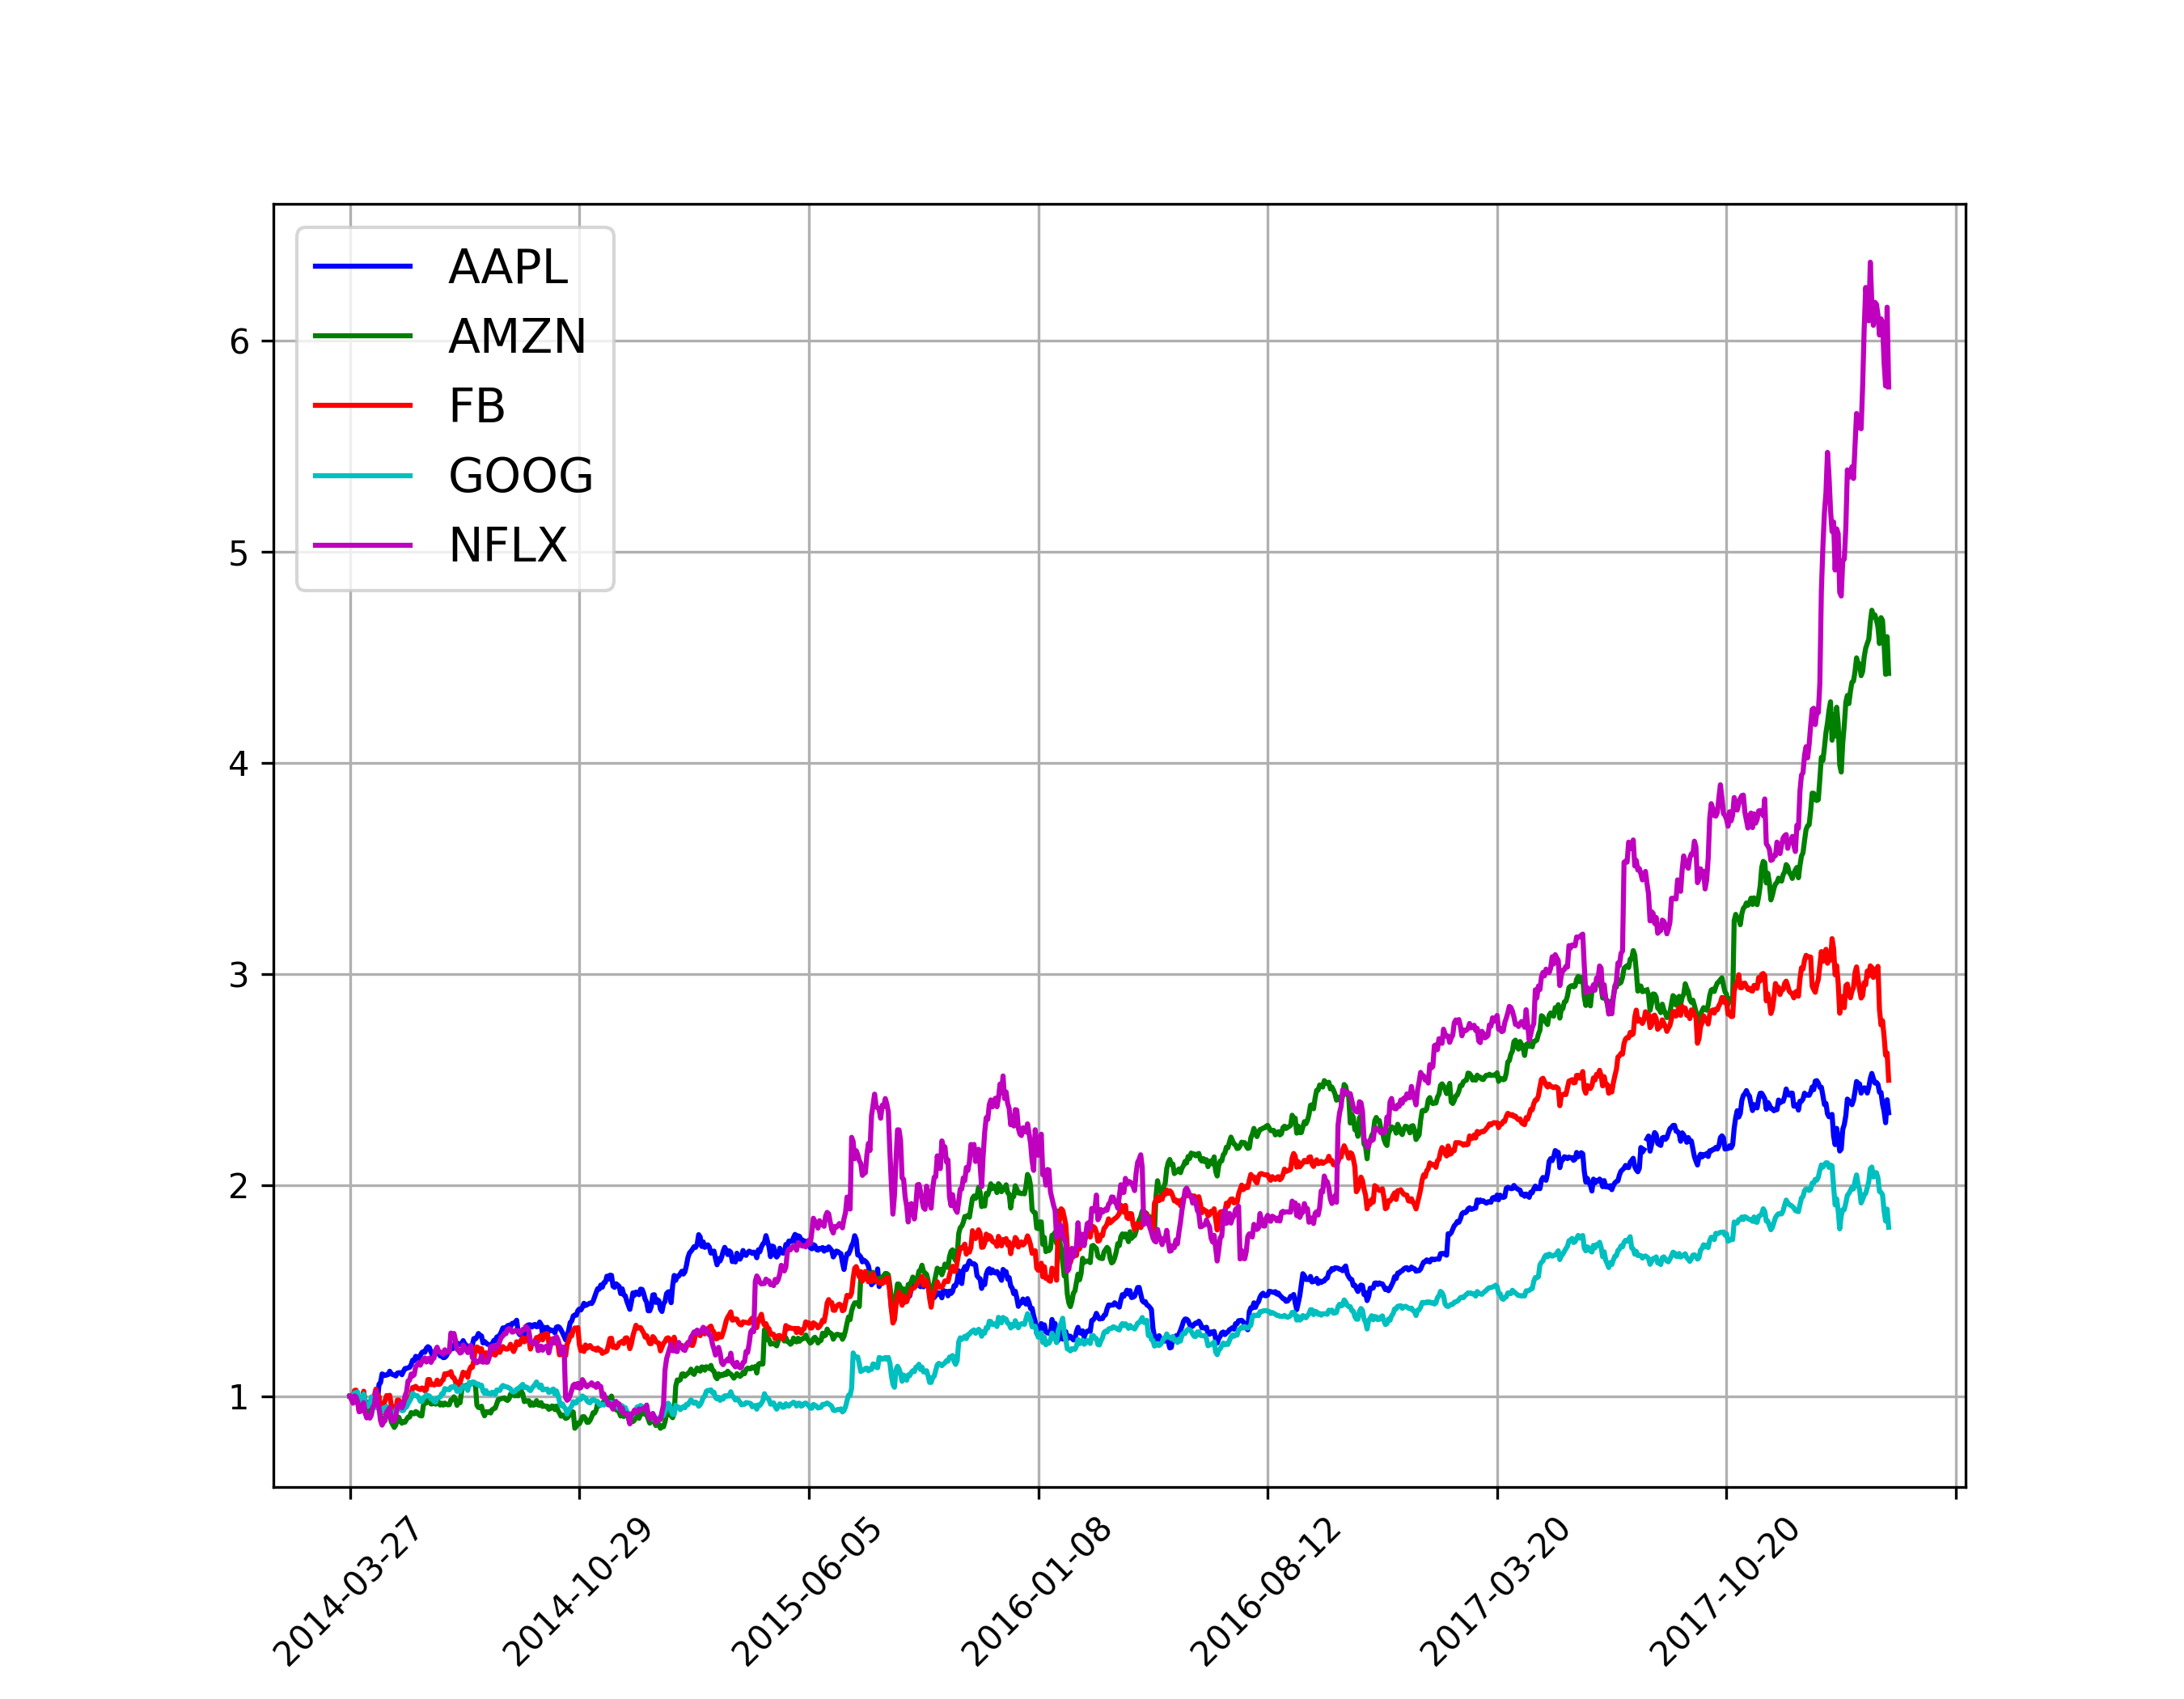
\includegraphics[width=0.7\textwidth]{figures/portfolio_sample}
\caption{Historical series of the closing price of five companies. To compare them, prices have been normalized to the first value in each series}
\label{fig:stocks}
\end{figure}

The main quantities (e.g. daily returns, covariance matrix,\ldots) can be easily computed with \texttt{pandas}.
Variances can be added across time intervals if return in one interval is uncorrelated with those in others. The correlation of returns across time intervals (called \emph{auto-correlation}) is in general close to zero for most assets. This means that variances will grow with the length of the forecast horizon and the risk will grow with the square root of the forecast horizon. 
Thus, a 5\% annual risk is equivalent to a 2.5\% risk over the first quarter or a 10\% risk over four years. 

This relationship can be used to “annualize” risk, i.e. standardize risk numbers to an annual period. The observed daily return standard deviation ($\sigma_{daily}$) can be converted to annual risk according to
\begin{equation}
\sigma_{yearly} = \sigma_{daily}\cdot\sqrt{252}
\end{equation}

\begin{ipython}
daily_returns = df.pct_change()
returns = daily_returns.mean()*252
print (returns)
\end{ipython}
\begin{ioutput}
AAPL    0.240921
AMZN    0.414775
FB      0.263708
GOOG    0.173464
NFLX    0.527628
dtype: float64
\end{ioutput}

\begin{ipython}
covariance = daily_returns.cov()*252
print (covariance)
\end{ipython}
\begin{ioutput}
          AAPL      AMZN        FB      GOOG      NFLX
AAPL  0.051967  0.025182  0.026075  0.022764  0.028064
AMZN  0.025182  0.085876  0.041196  0.039654  0.048576
FB    0.026075  0.041196  0.069723  0.036337  0.044753
GOOG  0.022764  0.039654  0.036337  0.052001  0.040630
NFLX  0.028064  0.048576  0.044753  0.040630  0.178332
\end{ioutput}
    
\subsection{Portfolio Simulation}
In order to "simulate" a portfolio of $n$ assets it is enough to throw $n$ random weights with the only constraint that they had to sum up to 1. 
In Figure~\ref{fig:mc_portfolio} a large number of simulated portfolios, each made of different proportion of the five assets mentioned above, are shown in a return vs volatility plot. 
Note that in these simulation no attempt of any optimization whatsoever has been made yet.

\begin{figure}[hbtp]
\centering
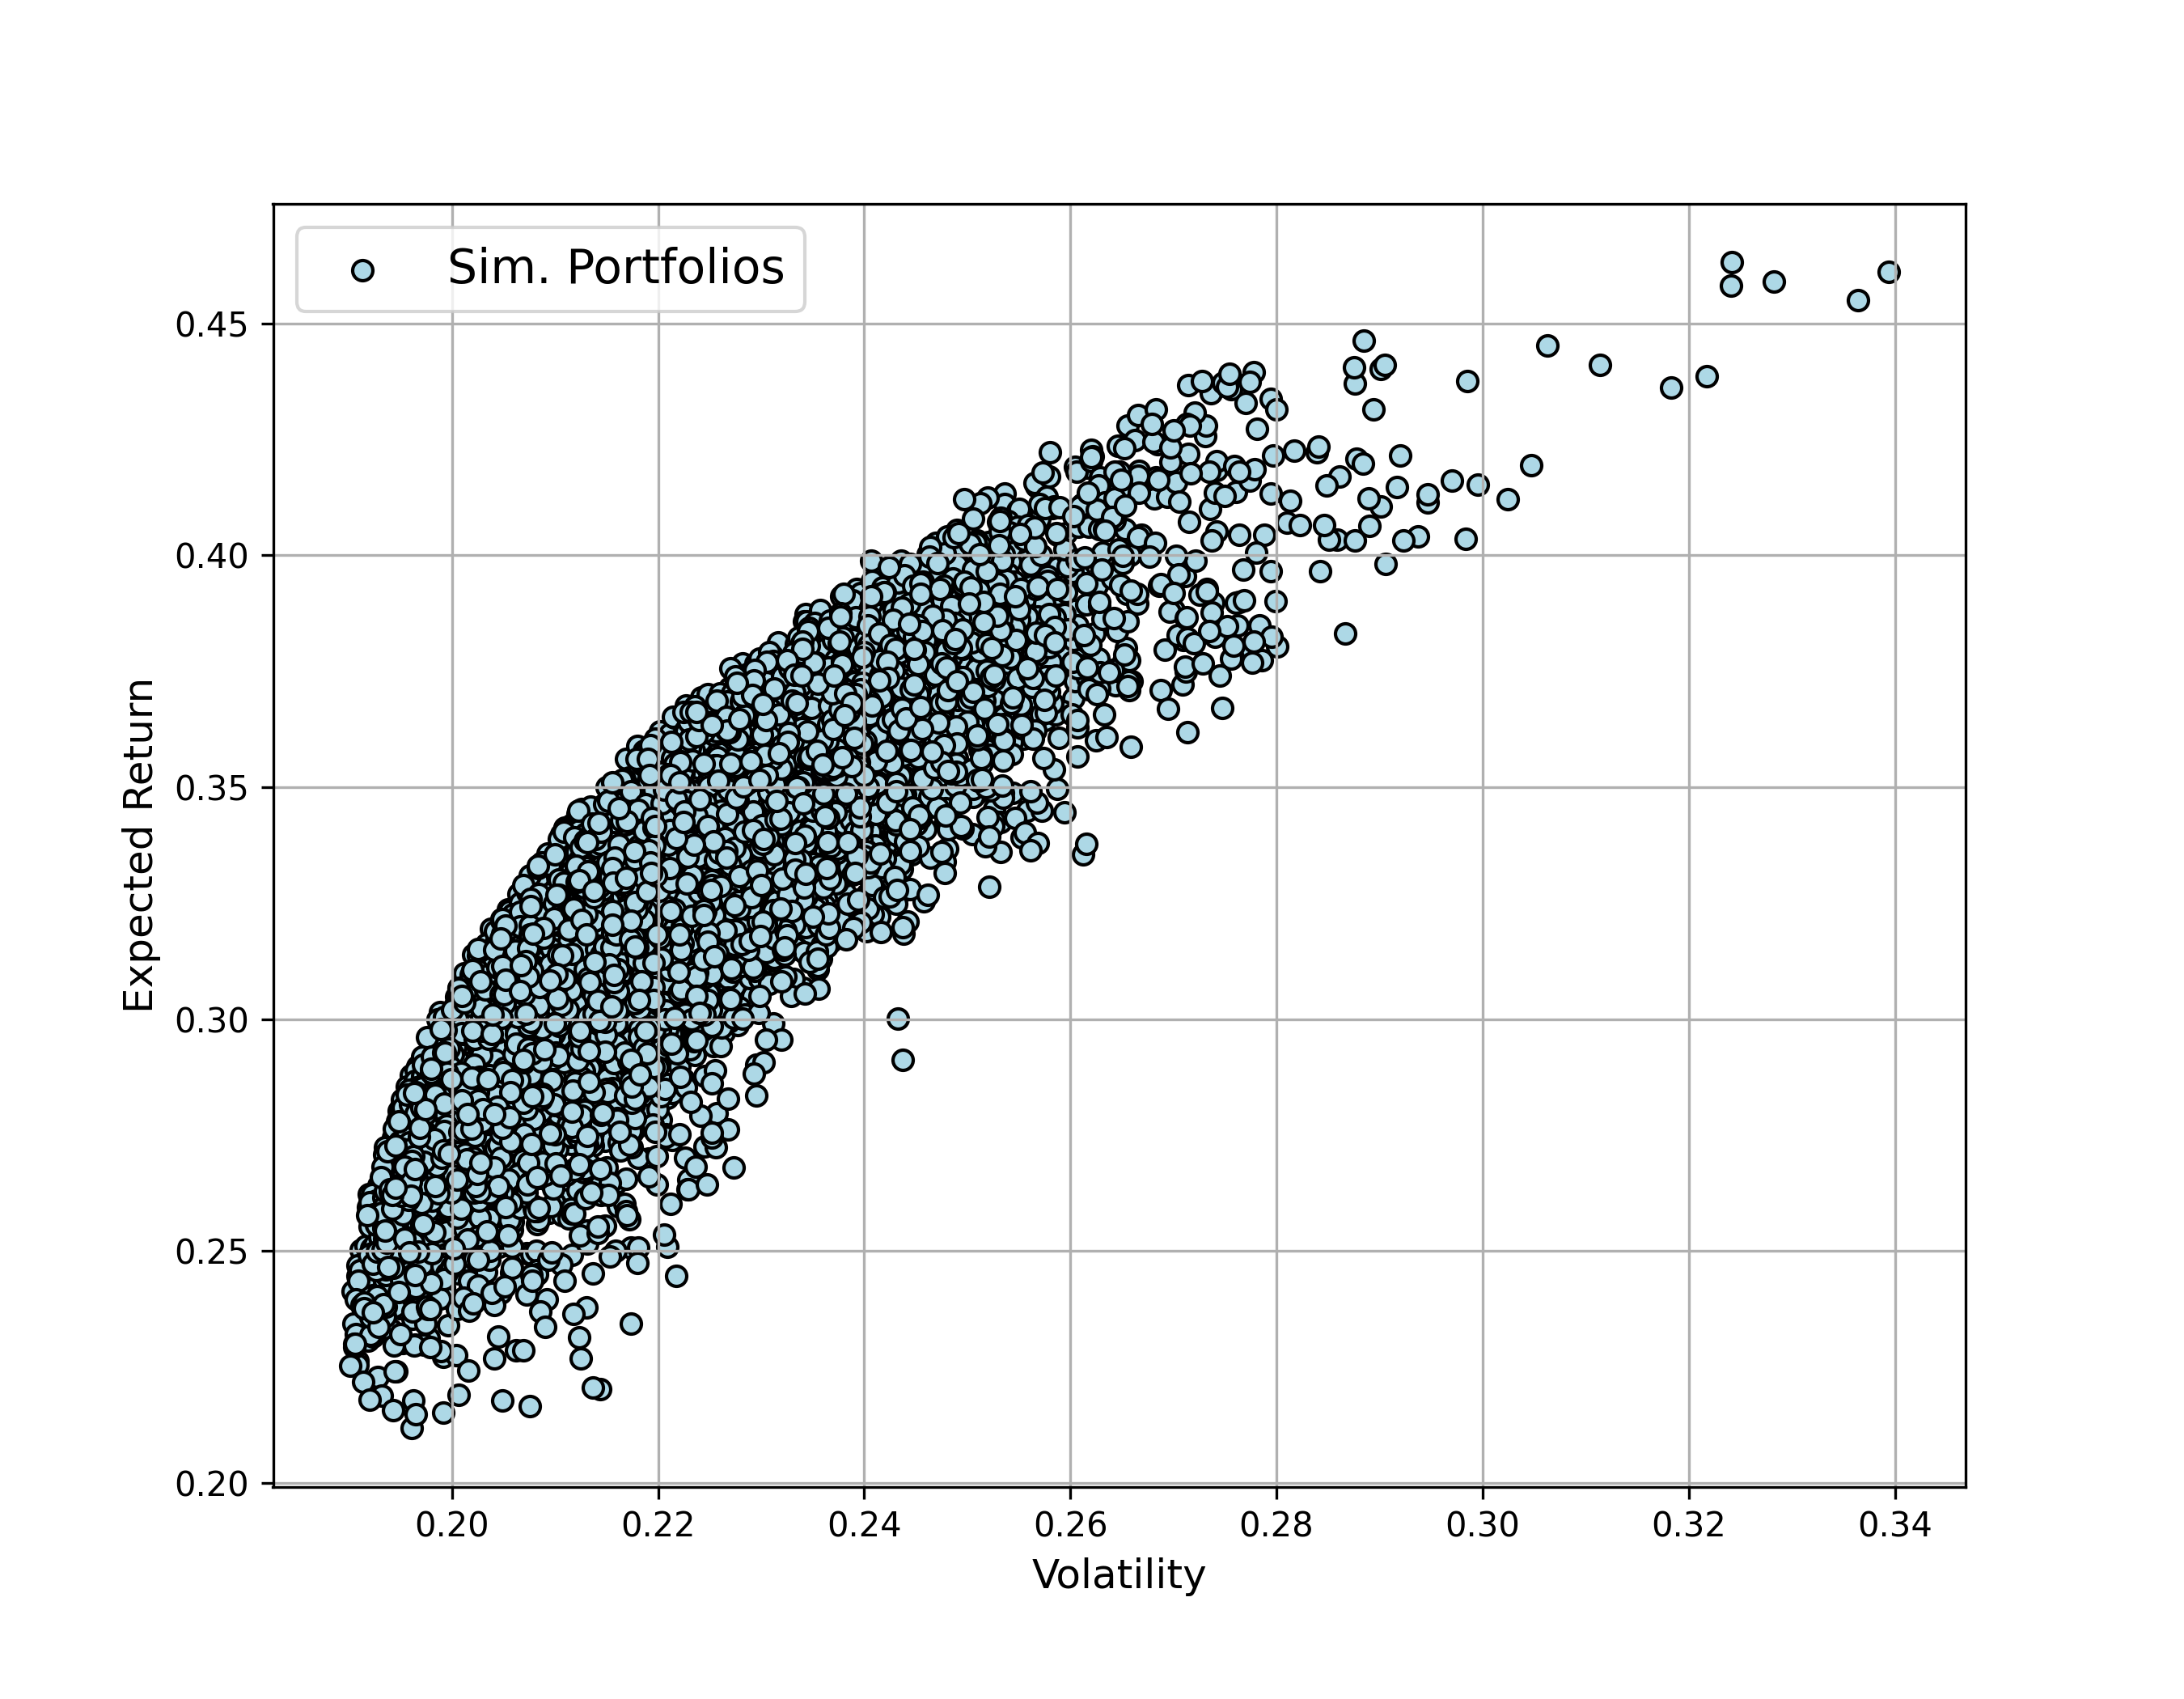
\includegraphics[width=0.7\textwidth]{figures/return_variance}
\caption{Scatter plot of expected return vs volatility of a large number of simulated portfolios.}
\label{fig:mc_portfolio}
\end{figure}

Investors may use \emph{short sales} in their portfolios (a portfolio is short in those stocks with negative weights). 
Although short selling extends the set of possible portfolios we are not going to consider it here.

\section{Optimization}\label{optimization}

MPT model states that \textbf{the weights of a portfolio should be chosen such that its volatility (or its variance) is minimized, given a certain level of return}. Alternatively weights can be found by maximizing the return given a certain level of risk. 
The application of this model reduces to a minimization problem: given the covariance matrix of the portfolio $\Sigma$, we need to find

\begin{equation}
\underset{\mathbf{w}}{\min}\{\sigma_p^2\} = \underset{\mathbf{w}}{\min}\{\mathbf{w}^T\Sigma\mathbf{w}\}
\end{equation}
with the constraints $\sum_{i}w_i = 1$ , $0 \le w_i \le 1$ and $\mathbf{w}\cdot\mathbf{R}=R_{\textrm{target}}$.

In \texttt{python} we have already seen how to solve minimization problems (see bootstrapping in Chapter~\ref{sec:swaps-and-bootstrapping}) so it is enough to repeat the same steps:

\begin{itemize}
\tightlist
\item define an objective function (i.e. the portfolio variance);
\item define the set of constraints;
\item set an initial guess for the weights;
\item run the algorithm with \texttt{scipy.optimize.minimize}.
\end{itemize}

\begin{ipython}
import numpy as np
from scipy.optimize import minimize

def sum_weights(w): 
    return np.sum(w) - 1

def min_risk(w, cov):
    return w.T.dot(cov.dot(w))

def target_return(w, returns, target_return): 
    return (returns.dot(w) - target_return)

num_assets = 5
constraints = [{'type': 'eq', 'fun': sum_weights},
               {'type': 'eq', 'fun': target_return, 'args':(returns, 0.25)}] 
bounds = tuple((0, 1) for _ in range(num_assets))
weights = [1./num_assets for _ in range(num_assets)]

opts = minimize(min_risk, weights, args=(covariance,),
                bounds=bounds, constraints=constraints)
print (opts)
print (f"Expected portfolio return: {returns.dot(opts.x):.3f}")
\end{ipython}
\begin{ioutput}
     fun: 0.03636340858846002
     jac: array([0.07251946, 0.07721784, 0.07324787, 0.07043841, 0.08025067])
 message: 'Optimization terminated successfully'
    nfev: 48
     nit: 8
    njev: 8
  status: 0
 success: True
       x: array([0.43988165, 0.10839598, 0.12863822, 0.29488199, 0.02820217])
       
Expected portfolio return: 0.250
\end{ioutput}

The optimization recommends to devote about 44\% of the portfolio to AAPL, about 10\% to AMZN, 12\% to FB and so on\ldots The expected return is 25\% as desired, with a variance of about 0.036 or, equivalently, a standard deviation of 0.19.

%In this example we based the model simply on straightforward statistical data derived from daily returns. However it could be possible, rather than just use historical data, to base this estimate on information about expected future performance of the asset.

There is no precise way for an investor to determine the “correct” trade off between risk and return. The desired higher expected return needs to be paid for with higher risk. Thus, one is frequently interested in looking at the relative distribution of the two.
In finance terminology, means to trace the \emph{efficient frontier of return and risk}. This can be done by solving the previous minimization for a variety of target returns.

The following example computes the efficient frontier plot (shown in Fig.~\ref{fig:efficient_frontier}) with the return ranging from 0.20 to 0.45.

\begin{ipython}
results = []    
for target in np.arange(0.20, 0.45, 0.005):
    constraints = ({'type': 'eq', 'fun': sum_weights},
                   {'type': 'eq', 'fun': target_return, 'args':(returns, target)})
    weights = [1./num_assets for _ in range(num_assets)]
    opts = minimize(min_risk, weights, args=(covariance,), 
                    bounds=bounds, constraints=constraints) 
    
    results.append((np.sqrt(opts.x.T.dot(covariance.dot(opts.x))),
                    returns.dot(opts.x))) 
\end{ipython}

\begin{figure}[htb]
\centering
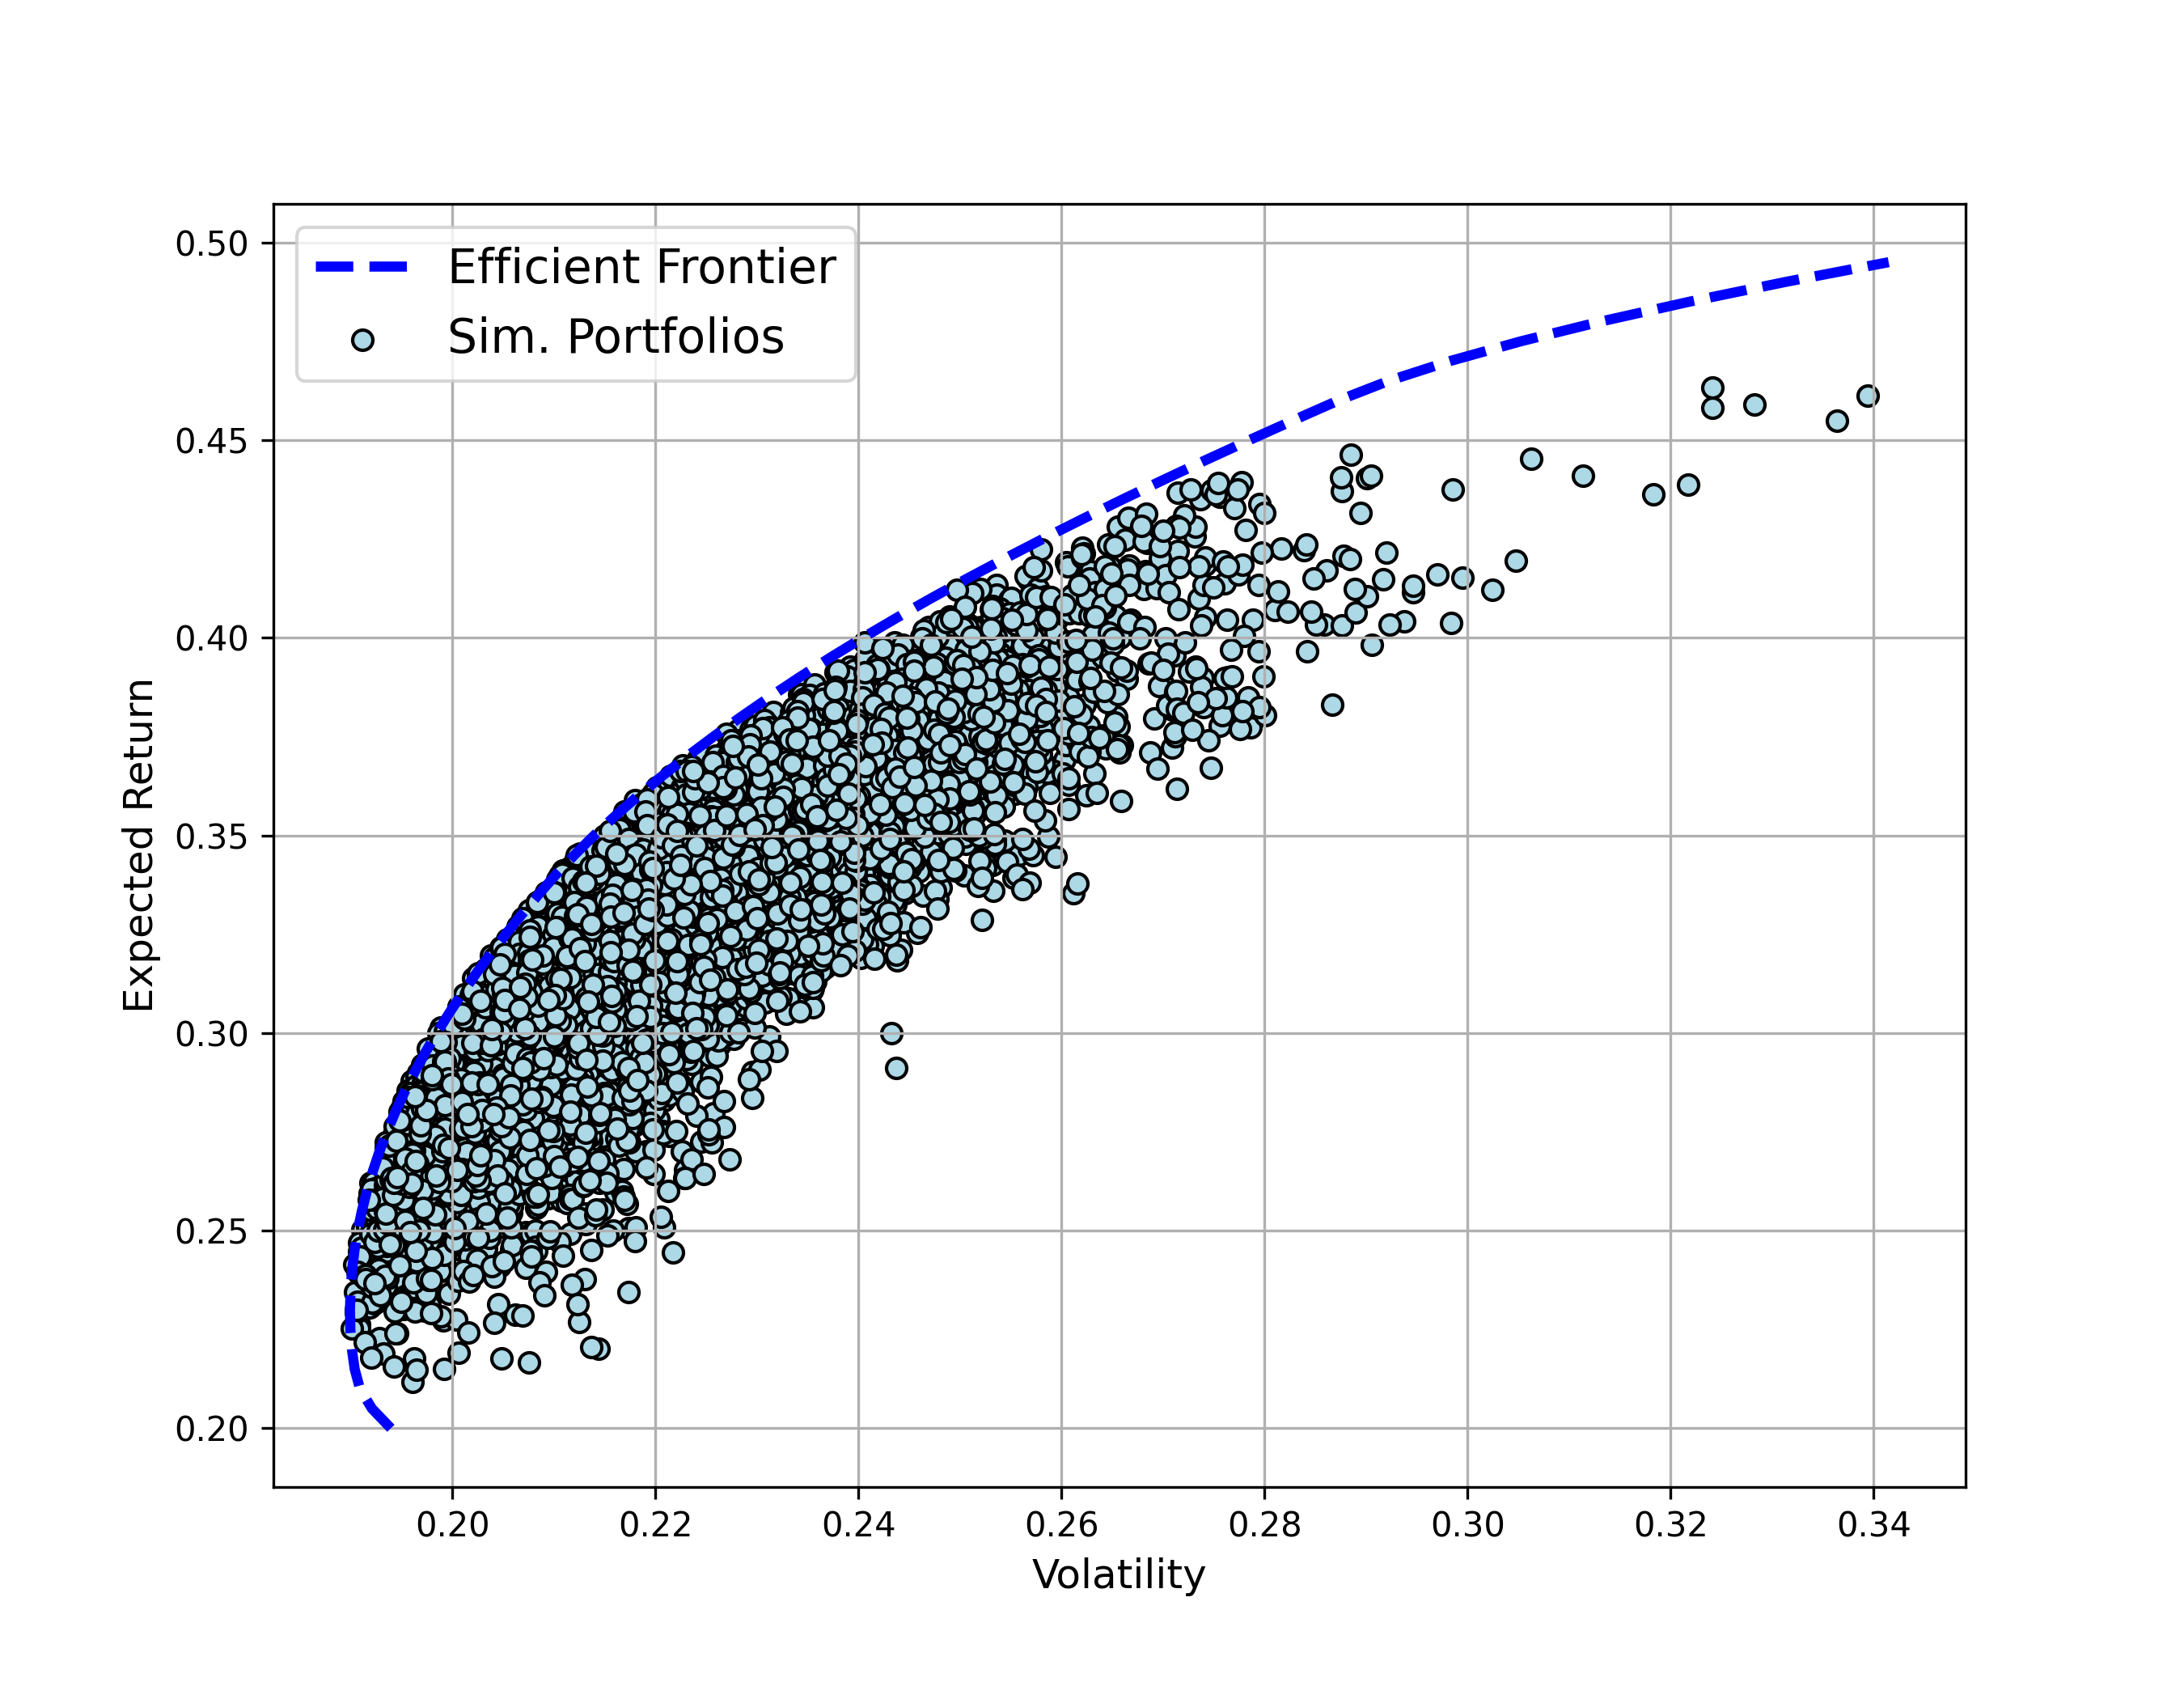
\includegraphics[width=0.7\textwidth]{figures/efficient_frontier}
\caption{Efficient frontier for our example portfolio obtained minimizing the the variance and requiring an expected return between 0.02 and 0.45.}
\label{fig:efficient_frontier}
\end{figure}

\emph{Efficient portfolios} offer investors the highest possible expected return for a given level of risk. 
An investor seeking high expected returns and low volatility should invest only in efficient portfolios and will choose from the set of efficient portfolios based on her risk tolerance.
    
\subsection{Limits of the Markowitz Model}
\label{limits-of-the-markowitz-model}

Despite the significant utility of the Markowitz theory, there are some major limitations in this model:

\begin{enumerate}
\tightlist
\item the tendency to produce extreme portfolios combining extreme shorts with extreme longs. As a result,portfolio managers generally do not trust these extreme weights. This problem is typically caused by
estimation errors in the mean return vector and covariance matrix;
\item the portfolio weights tend to be extremely sensitive to very small changes in the expected returns. For example, even a small increase in the expected return of just one asset can dramatically alter the optimal composition of the entire portfolio;
\item the presence of heavy tails in the return distributions can result in significant errors in covariance estimates as well.
\end{enumerate}

Extensions of the Markowitz model are defined in~\cite{bib:post_modern_theory} and~\cite{bib:black_litterman}, although they are beyond the scope of these lectures. 
    
\subsection{Portfolios with a Risk-Free Asset}
\label{portfolios-with-a-risk-free-asset}

When one of the investments available is a risk-free asset, then the efficient frontier transform to a particularly simple form. The risk–return combinations of the risk-free investment and a risky portfolio lie on a straight line connecting the two investments: the \emph{capital allocation line} (CAL). The slope of the CAL measures the trade off between risk and return: a higher slope means investors receive a higher expected return in exchange for taking on more risk.

The capital allocation line aids investors in choosing how much to invest in a risk-free asset and one or more risky assets.

The simplest example of such kind of portfolios is the one containing only two assets: a risk-free Treasury bill and a stock. Assume that the expected return of the Treasury bill is \(\mathbb{E}(R_f)=3\%\) (its risk is 0\%). Further, assume that the expected return of the stock is \(\mathbb{E}(R_r)=10\%\) and its standard deviation is \(\sigma_r=20\%\). The question that needs to be answered for any individual investor is how much to invest in each of these assets.

The expected return (\(\mathbb{E}(R_p)\)) of this portfolio is calculated as follows:

\begin{equation*} 
\mathbb{E}(R_p) = \mathbb{E}(R_f)\cdot w_f + \mathbb{E}(R_r)\cdot (1- w_f) 
\end{equation*}
where \(w_f\) is the relative allocation to the risk-free asset.

The calculation of this portfolio risk is simple because the standard deviation of the Treasury bill is 0\%. Thus

\begin{equation*} 
\sigma_p = (1-w_f)\cdot \sigma_r 
\end{equation*}
In this simple example, if an investor invested 100\% into the risk-free asset (\(w_f=1\)), the expected return would be 3\% and the risk of the portfolio would be 0\%. Otherwise, investing 100\% into the stock (\(w_f=0\)) would give an investor an expected return of 10\% and a portfolio risk of 20\%. If the investor allocated 25\% to the risk-free asset and 75\% to the risky asset, the portfolio expected return and risk calculations would be

\begin{equation*}
\begin{gathered}
\mathbb{E}(R_p) = (3\% \cdot 25\%) + (10\% \cdot 75\%) = 0.75\% + 7.5\% = 8.25\% \\
\sigma_p = 75\% \cdot 20\% = 15\% 
\end{gathered}
\end{equation*}
\noindent
If you plot these three points they lay on a line.

If we added a risk-free asset, with an expected return of 10\%, to the five risky ones considered so far we could repeat the Markowitz minimization to determine the efficient frontier of the resulting portfolio. 

\begin{ipython}
num_assets = 6
returns_rf = np.append(returns.values, 0.10)
cov_rf = np.column_stack((covariances.values, np.array([0, 0, 0, 0, 0])))
cov_rf = np.row_stack((cov_rf, np.array([0, 0, 0, 0, 0, 0])))
print (cov_rf)

result_rf = []

for t_ret in np.arange(0.1, 0.4, 0.01):
    weights = [1/n_assets for _ in range(num_assets)]
    bounds = [(0, 1) for _ in range(num_assets)]
    constraints = [{'type':'eq', 'fun':sum_weights},
                   {'type':'eq', 'fun':target_return, 'args':(returns_rf, t_ret)}]

    opts = minimize(min_risk, weights, bounds=bounds, 
                    constraints=constraints, args=(cov_rf))

    result_rf.append((np.sqrt(risk(opts.x, covariance)),
                      returns.dot(opts.x)))
\end{ipython}
\begin{ioutput}
[[0.05190222 0.02503721 0.02573699 0.02245413 0.02775968 0.        ]
 [0.02503721 0.08583929 0.04102487 0.03950122 0.04841167 0.        ]
 [0.02573699 0.04102487 0.06955025 0.03612685 0.04452847 0.        ]
 [0.02245413 0.03950122 0.03612685 0.05179662 0.04038995 0.        ]
 [0.02775968 0.04841167 0.04452847 0.04038995 0.17829826 0.        ]
 [0.         0.         0.         0.         0.         0.        ]]
\end{ioutput}

\begin{figure}[htb]
\centering
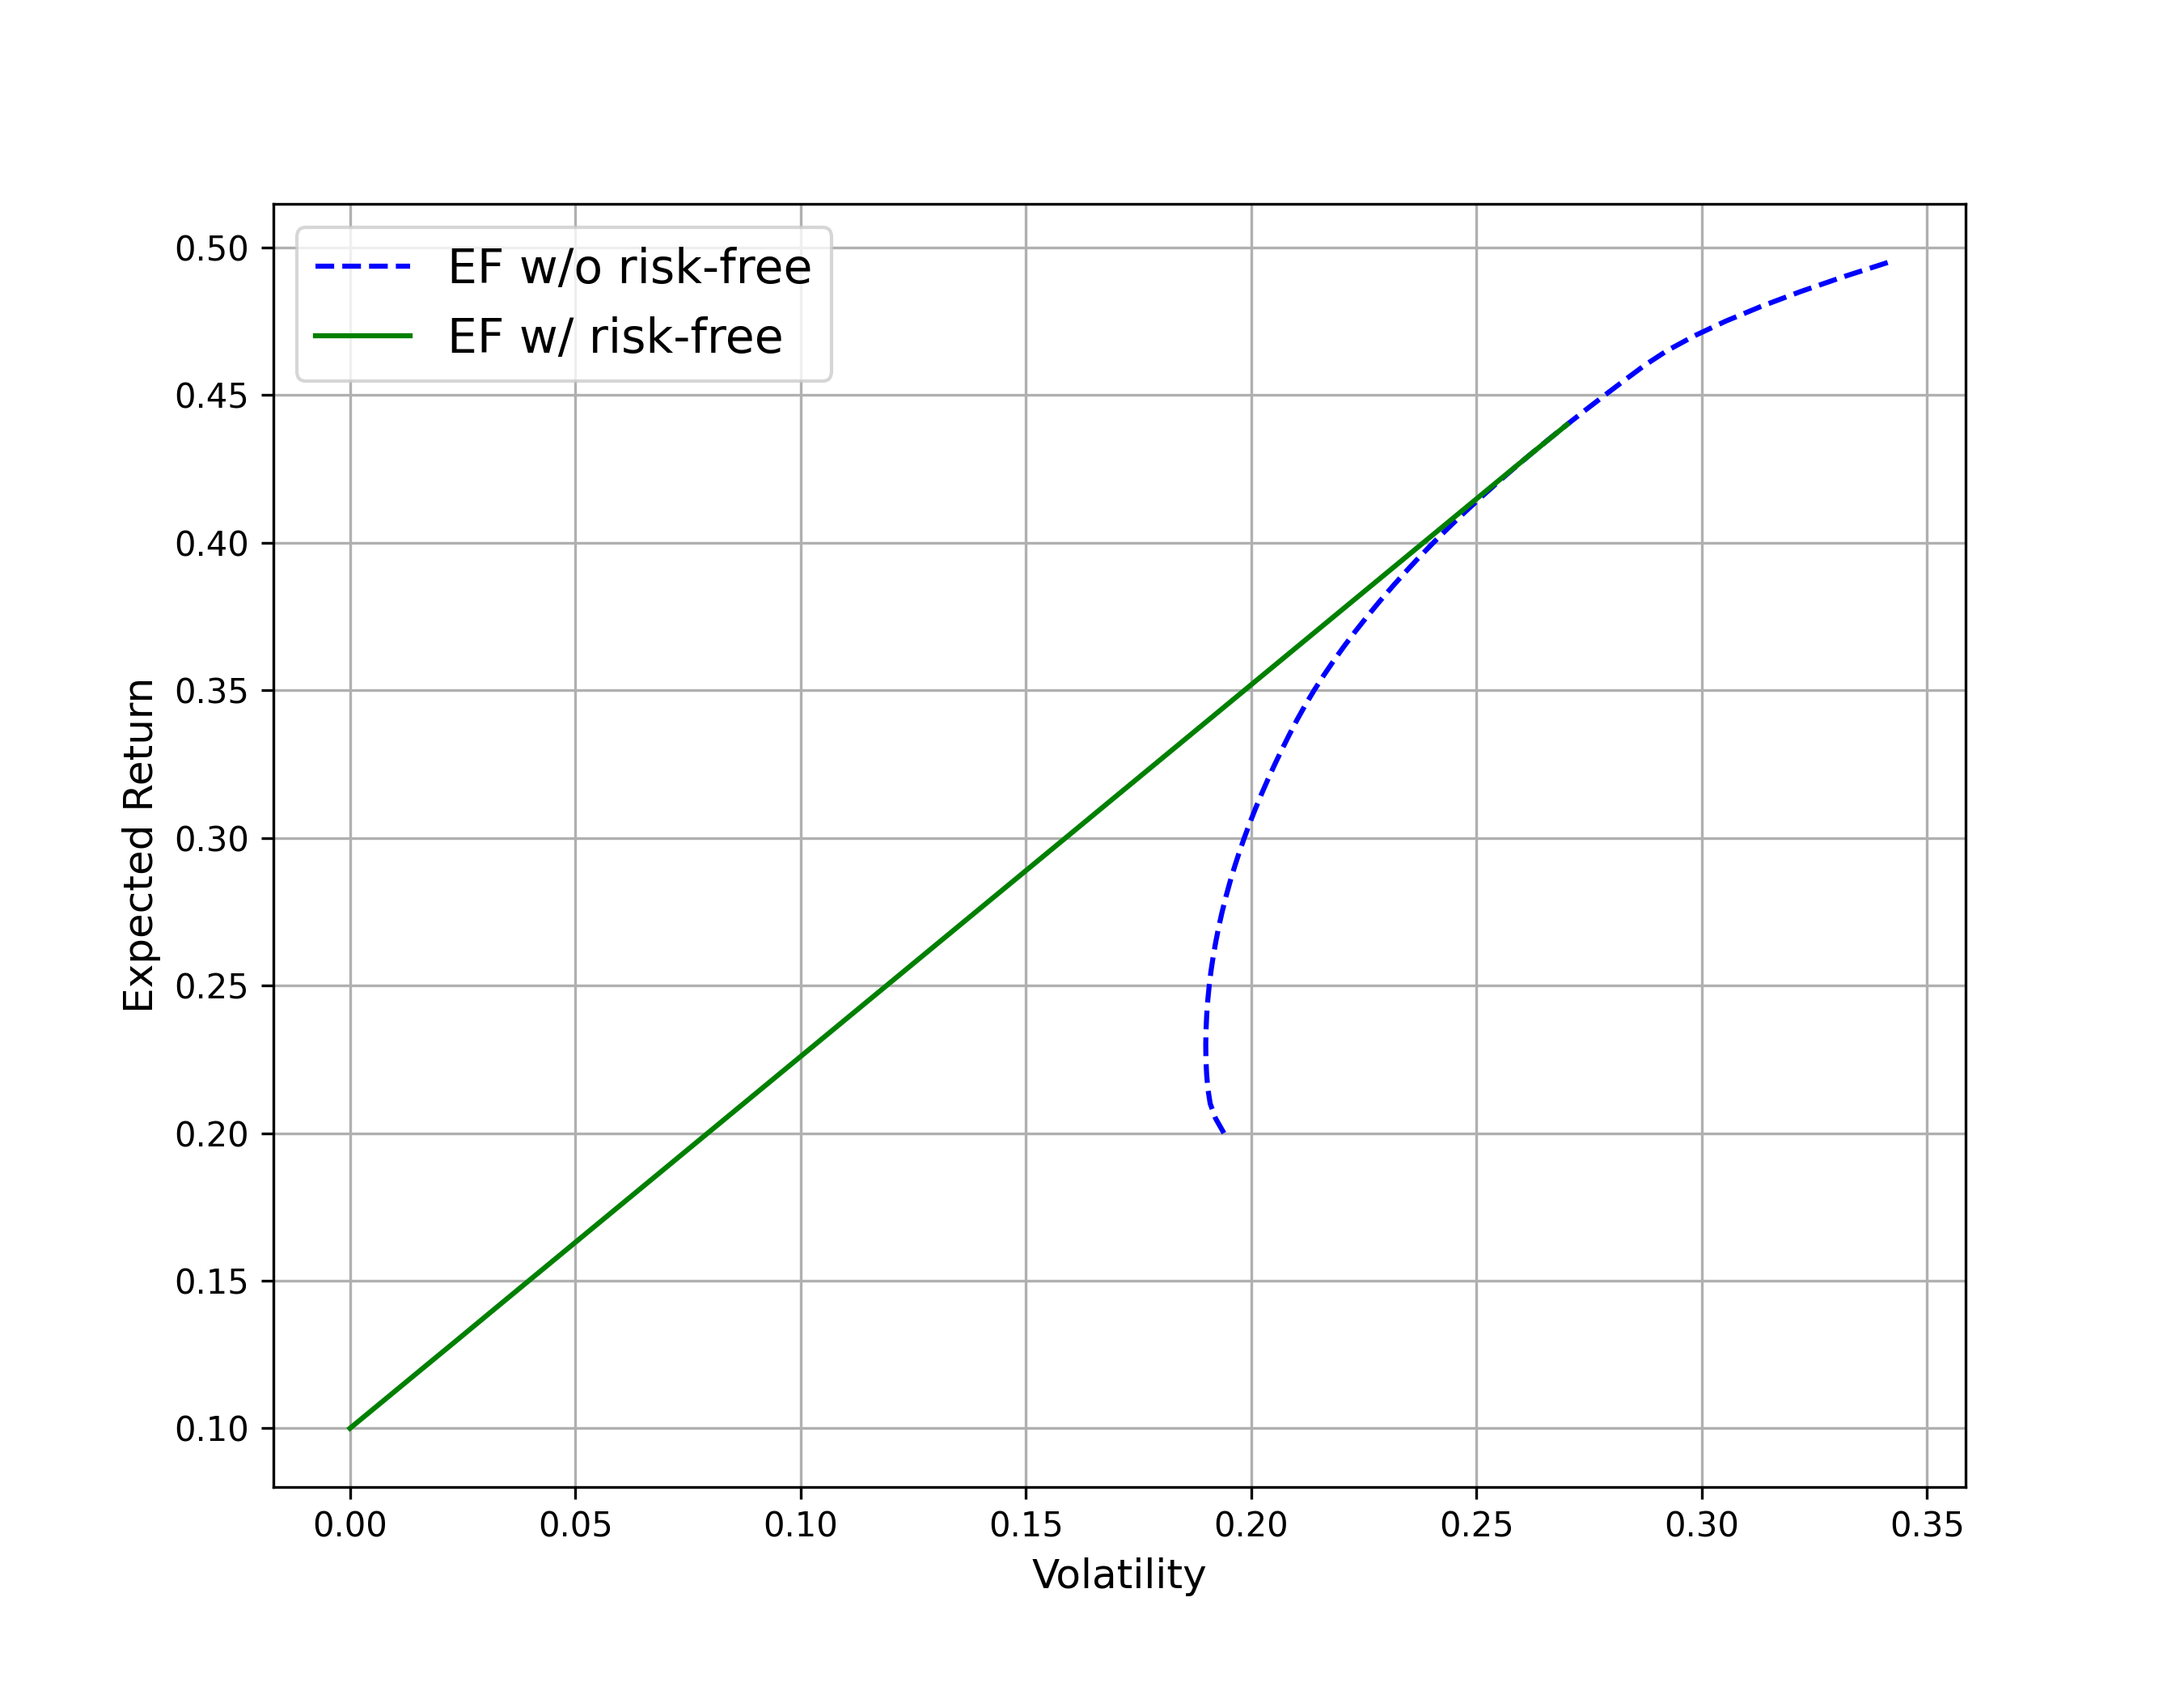
\includegraphics[width=0.7\textwidth]{figures/cal}
\caption{Comparison of efficient frontier with a risk-free asset (red) and with risky asset only (blue).}
\label{fig:cal}
\end{figure}
    
As expected the efficient frontier has become a straight line, tangent to the frontier of the risky assets (Fig.~\ref{fig:cal}). When the target is 10\% the entire investment is allocated to the risk-free asset, as the target increases the fraction of risky assets grows proportionally to the volatility. 

It is important to notice that in general the relative proportions among the risky investments do not change with or without the risk-free asset. Only the allocation between the risk-free and the risky parts varies.

\section{The Sharpe Ratio}
\label{the-sharpe-ratio}
The goal of an investor who is seeking to earn the highest possible expected return for any level of volatility is to find the portfolio that generates the steepest possible line when combined with the risk-free investment. This line slope is called the \emph{Sharpe ratio} of the portfolio.

For a portfolio of risky assets let be

\begin{itemize}
\tightlist
\item \(R_r\) its expected return;
\item \(\sigma_r\) its standard deviation in return;
\item \(r_f\) the return of a risk-free asset.
\end{itemize}

A plausible single measure of attractiveness of a portfolio (as opposed to the two measures, risk and return proposed by MPT model) is the Sharpe ratio:

\begin{equation} 
\mathcal{S} = \cfrac{R_r - r_f}{\sigma_r} 
\end{equation}
\noindent
In words, it measures how much additional return is achieved for the higher risk taken on, relative to investing all in the risk-free asset. 

The portfolio that maximizes this ratio has some interesting properties. Suppose that

\begin{itemize}
\tightlist
\item
  \(R_\textrm{target}\) the desired target return;
\item
  \(w_r\) the fraction of wealth placed in the portfolio (the rest placed in the risk-free asset).
\end{itemize}
\noindent
To meet the target return the weights need to be chosen such that:

\begin{equation*} 
(1 - w_r) * r_f + w_r * R_r =R_\textrm{target} 
\end{equation*}
\noindent
The standard deviation of the investment is: \(w_r\cdot \sigma_r\). Solving for \(w_r\) in the equation above, we get:

\begin{equation*} 
	w_r = \cfrac{R_\textrm{target} - r_f}{R_r - r_f} 
\end{equation*}
Thus, the standard deviation of the portfolio is:

\begin{equation*} 
w_r\cdot \sigma_r = \left(\cfrac{R_\textrm{target} - r_f}{R_r - r_f}\right)\cdot \sigma_r 
\end{equation*}
Minimizing the portfolio standard deviation means:

\begin{equation} 
\textrm{min}\left\{\cfrac{R_\textrm{target} - r_f}{R_r - r_f}\cdot \sigma_r\right\} = \textrm{min}\left[\cfrac{R_\textrm{target} - r_f}{\mathcal{S}}\right]
\end{equation}

Since in the above formula both $R_{\textrm{target}}$ and $r_f$ are constant, the minimization is equivalent to the maximization of the denominator of the expression, hence of the Sharpe ratio $\mathcal{S}$.

\begin{equation} 
\textrm{min}\left\{\cfrac{R_\textrm{target} - r_f}{\mathcal{S}}\right\}
\implies\textrm{max}\left\{\cfrac{R_r - r_f}{\sigma_r}\right\}
\end{equation}

So, regardless of investor risk/return preference, \emph{the investment should go in the portfolio that maximizes the Sharpe ratio}, because it will be the one that minimize the risk (i.e. standard deviation) and maximize the return at the same time.

Let's compute the Sharpe portfolio with our sample.

\begin{ipython}
num_assets = 5
rf_asset_return = 0.10

def sharpe_ratio(w, returns, rf_asset_return, cov): 
    p_ret = returns.dot(w)
    p_var = np.sqrt(w.T.dot(cov.dot(w)))
    ratio = -(p_ret - rf_asset_return) / p_var
    return ratio

constraints = ({'type': 'eq', 'fun': sum_weights})
bounds = tuple((0, 1) for asset in range(num_assets))
weights = [1./num_assets for _ in range(num_assets)]
opts = minimize(sharpe_ratio, weights, args=(returns, rf_asset_return, covariance),
                bounds=bounds, constraints=constraints)
print (opts)
print ("Sharpe ratio: ", -opts.fun)
\end{ipython}
\begin{ioutput}
     fun: -1.259317843917775
     jac: array([-0.37875983, -0.37936528, -0.26915939,  0.02855796, -0.37932488])
 message: 'Optimization terminated successfully'
    nfev: 36
     nit: 6
    njev: 6
  status: 0
 success: True
       x: array([1.19754346e-01, 5.43974190e-01, 5.20417043e-18, 1.22298005e-16,
                 3.36271464e-01])

Sharpe ratio:  1.259317843917775)
\end{ioutput}

Figure~\ref{fig:sharpe_ratio} shows the optimization results. Notice that in general the relative proportions of the stocks are the same as in the previous case (at the same level of return) where we explicitly included a risk free asset (0.12, 0.54, 0., 0., 0.33).

\begin{figure}[htb]
\centering
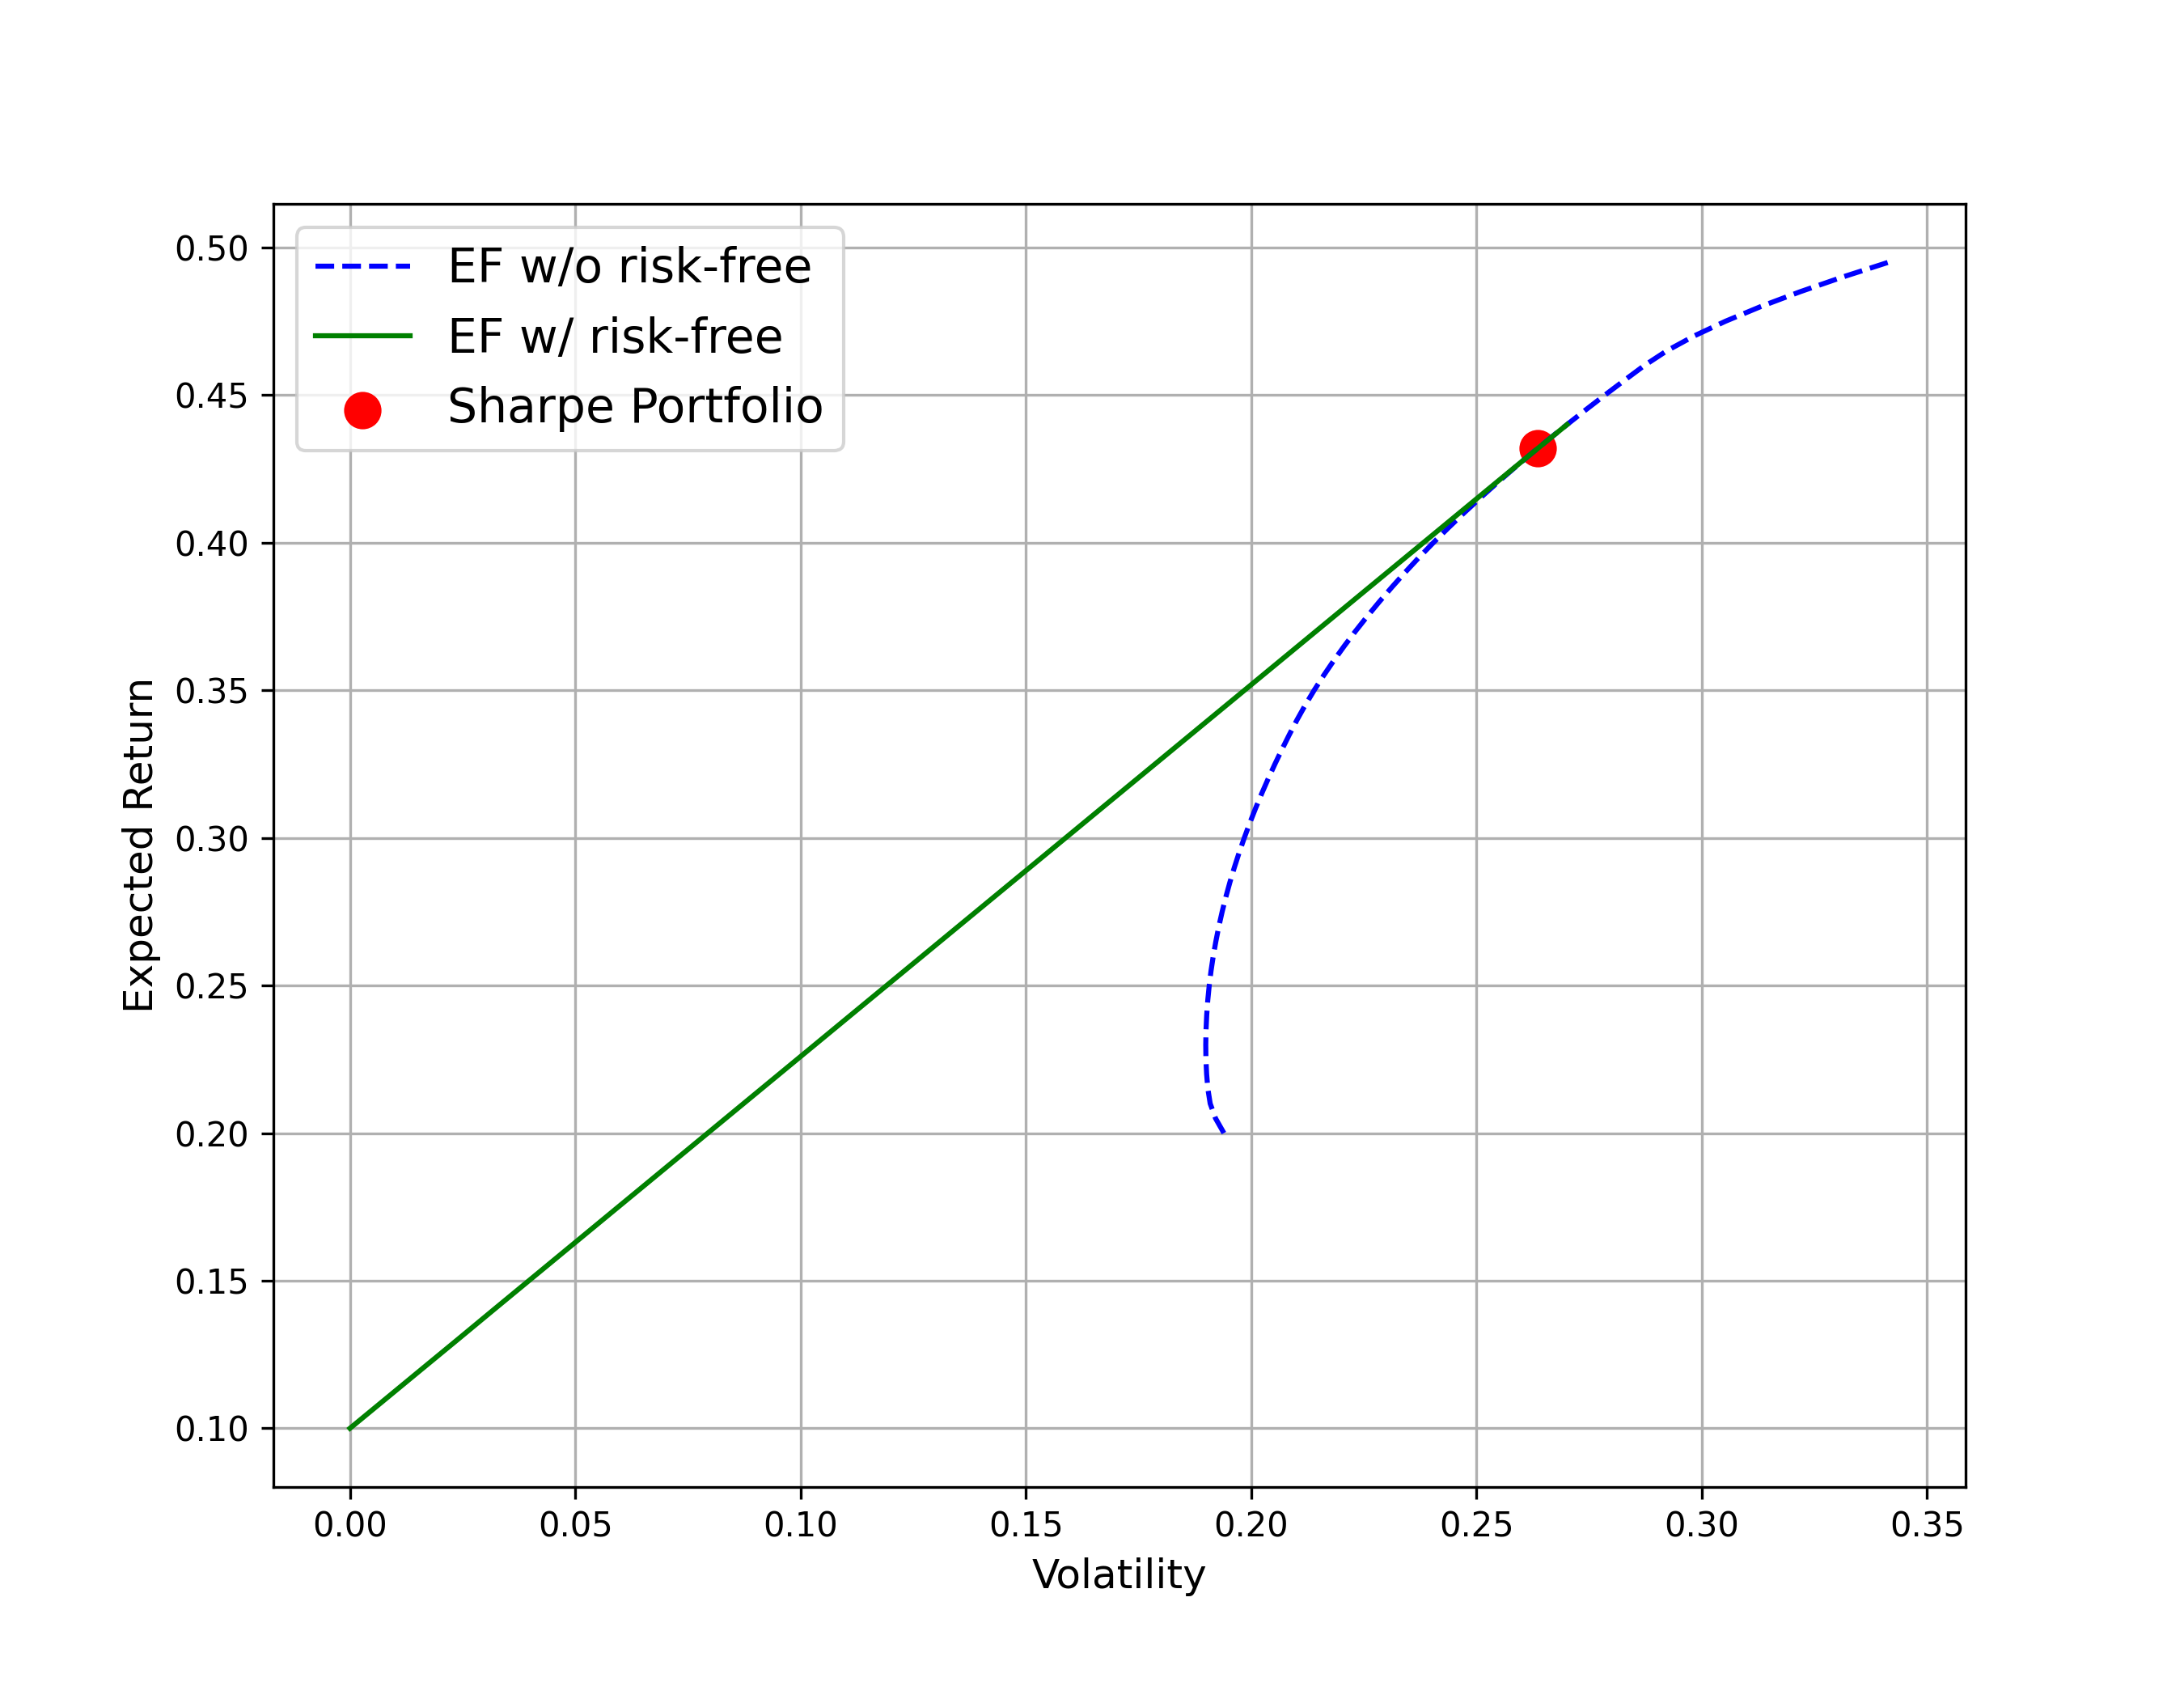
\includegraphics[width=0.7\textwidth]{figures/sharpe_ratio}
\caption{Sharpe portfolio (green cross) compared to the efficient frontier with a risk-free asset (red) and with risky asset only (blue).}
\label{fig:sharpe_ratio}
\end{figure}

So using the Sharpe ratio gives a portfolio that is on the efficient frontier, and gives the maximum return relative to putting all our money in the risk-free asset so is on the CAL too. Graphically it sits in the only place that belongs to both curves: the tangent point.

Usually, any Sharpe ratio greater than 1.0 is considered acceptable to good by investors. A ratio higher than 2.0 is rated as very good. A ratio of 3.0 or higher is considered excellent. A ratio under 1.0 is sub-optimal.

\section{Portfolio Diversification}

A security total risk can be divided into \emph{unsystematic}, the risk portion peculiar to the company that can be diversified away, and systematic, the non-diversifiable portion that is related to the movement of the stock market and is therefore unavoidable. 

Diversification is a common topic in portfolio construction and allows to combine risky stocks so that the resulting portfolio is less risky than the sum of its components. Although such diversification is a familiar notion, it may be worthwhile to review the manner in which diversification reduces risk.

Suppose there are two companies located on an isolated island whose chief industry is tourism. One company manufactures suntan lotion; its stock predictably performs well in sunny years and poorly in rainy ones. The other company produces umbrellas; its stock performs equally poorly in sunny years and well in rainy ones. Each company earns a 12\% average return.

In purchasing either stock, investors incur a great amount of risk because of the price variability driven by fluctuations in weather conditions. Investing half the funds in the suntan lotion stock and half in the umbrella manufacturer stock, however, results in a return of 12\% regardless of which weather condition prevails. Portfolio diversification thus transforms two risky stocks, each with an average return of 12\%, into a risk-less portfolio certain of earning the expected 12\%.

Unfortunately, the perfect negative relationship between the returns on these two stocks is very rare in real world. To some extent, corporate securities move together, so complete elimination of risk through simple portfolio diversification is impossible. However, as long as some lack of parallelism in the returns of securities exists, diversification will always reduce risk.
Empirical studies have demonstrated that risk can be virtually eliminated in portfolios of 30 to 40 randomly selected stocks. Of course, if investments are made in closely related industries, more securities are required to eradicate it.

When using the standard variation of the portfolio return as a measure of the risk, as in the Markowitz model, it is easy to show how diversification allows to reduce the risk. 
Indeed the standard deviation of a portfolio is not the weighted average of the standard deviations of the component stocks.
For example, suppose the correlation between the return of stocks 1 and 2 is $\rho_{12}$. If the portfolio is equally weighted then

\begin{equation}
\sigma_{P} = \sqrt{(0.5\cdot\sigma_1 )^2 + (0.5\cdot\sigma_2 )^2 + 2\cdot(0.5\cdot\sigma_1)(0.5\cdot\sigma_2)\rho_{12}} < (0.5\cdot\sigma_1 ) + (0.5\cdot\sigma_2 )
\end{equation}

The inequality holds unless $\rho_{12}=1$, so in general, for risk, the whole is less than the sum of its parts. 
This is the key to portfolio diversification.

Figure~\ref{fig:diversification} shows the risk of a portfolio made up of IBM and General Electric stocks against the fraction of GE stocks in the portfolio. The curved line represents the risk of the portfolio; the straight line is the sum of the two contributions. The risk of GE is 27.4\% per year, the risk of IBM is 29.7\% per year, and the two are 62.9\% correlated. The gap between the lines is an indication of the benefit of diversification in reducing risk.

\begin{figure}[htb]
\centering
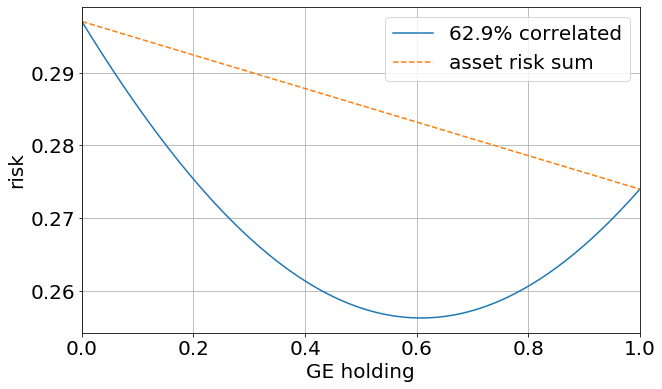
\includegraphics[width=0.7\textwidth]{figures/diversification}
\caption{Risk of a portfolio made up from IBM and General Electric against the fraction of GE stock in the portfolio. The curved line represents the risk of the portfolio; the straight line represents the sum of the two single risks.}
\label{fig:diversification}
\end{figure}

%We can see the power of diversification in another example. Given a  portfolio of $N$ stocks, each with risk $\sigma$ and uncorrelated returns, the risk of an equal-weighted portfolio of these stocks will be
%\begin{equation}
%\sigma_P = \cfrac{\sigma}{\sqrt{N}}
%\end{equation}
%
%Assume now that the correlation between the returns of all pairs of stocks is equal to $\rho$. Then the risk of an equally weighted portfolio is:
%\begin{equation}
%\sigma_P = \sigma\cdot\sqrt{\cfrac{1+\rho(N-1)}{N}};\quad \lim_{N \to +\infty} \sigma_P = \sigma\cdot\sqrt{\rho}
%\label{eq:risk_correlation}
%\end{equation}
%which can be further simplified when considering a portfolio contains a very large number of correlated stocks
%
%To get a feel for this, consider the example of an equal-weighted portfolio of the 20 Major Market Index constituent stocks. In December 1992, these stocks had an average risk of 27.8\%, while the equal-weighted portfolio has a risk of 20.4\%. Equation~\ref{eq:risk_correlation} then implies an average correlation between these stocks of 0.52. 

%As we have already seen no measure of unsystematic risk appears in the risk premium, of CAPM model, since it is assumed that diversification has eliminated it.
%
%In the Markowitz model instead diversification is achieved by seeking to combine in a portfolio assets with returns that are less than perfectly positively correlated, in an effort to lower portfolio risk (variance) without sacrificing return, through the reduction of the correlation matrix $\Sigma$.


An \emph{utility function} $u(x)$ is a function of wealth ($x$) that quantifies the ``happiness'' level of the investor. Typically this function has $u'(x) > 0$ and $u''(x) < 0$. The first condition reflects the simple concept that ``the more I have the happier I am''. The latter instead will be described later on in this Section.

In real life, the future wealth level will be uncertain, so we would use a random variable $X$ as the input of the utility function, leading us to the study of its expectation. First of all, it must be noticed that in general $\mathbb{E}[u(X)] \neq u(\mathbb{E}[X])$.
Since investors care for the utility we should prefer a random variable such that $\mathbb{E}[u(X)]$ is maximized.

%From the Jensen’s inequality we get that $\mathbb{E}[u(X)] < u (\mathbb{E}[X])$. Indeed
Using a simple Taylor expansion around the value $\mathbb{E}[X]$:
\begin{equation*}
u(X) = u (\mathbb{E}[X]) + u'(\mathbb{E}[X]) (X − \mathbb{E}[X]) + \frac{1}{2}u''(\mathbb{E}[X]) (X − \mathbb{E}[X])2 + \ldots
\end{equation*}

If we take the expectation of both sides, assuming $u'' < 0$,
\begin{equation*}
  \begin{aligned}
  \mathbb{E}[u(X)] &= u(\mathbb{E}[X]) + u'(\mathbb{E}[X]) \mathbb{E}[X − \mathbb{E}[X]] + \frac{1}{2}u''(\mathbb{E}[X]) \mathbb{E}(X − \mathbb{E}[X])^2 + \ldots\\
  &= u (\mathbb{E}[X]) + \frac{1}{2}u'' (\mathbb{E}[X]) Var(X) + \ldots < u (\mathbb{E}[X])
  \end{aligned}
\end{equation*}
If we let $X$ to be the realized return of certain investment, the investors’ goal would be to maximize the expected utility, and from the last equation above it seems
that we should maximize the expected value of the return ($\mathbb{E}[X]$) and minimize the variance of the return ($Var(X)$) at the same time. \emph{This is what is contained in Markowitz portfolio theory}.
But this result shows that optimizing the return of the portfolio can be viewed as maximizing the utility for the investor. The
advantage of the utility approach is that now we can use different utility functions for different investors’ preferences, mostly about their preferences towards risk.

For example assume $u(x) = 1−e^{−x}$ and $X$ is a normal random variable. Then we find
\begin{equation*}
  \mathbb{E}[u(X)] = 1 − \mathbb{E}[e^{−X}] = 1 − e^{−\mathbb{E}[X]+ \frac{1}{2}2Var(X)}
\end{equation*}

Since the exponential is an increasing function, the following are equivalent:
\begin{equation*}
  \max \mathbb{E}[u(X)] \equiv \min e^{−\mathbb{E}[X]+ \frac{1}{2}Var(X)} \equiv \min\left[−\mathbb{E}[X] + \frac{1}{2}Var(X)\right] \equiv \max\left[\mathbb{E}[X] − \frac{1}{2}Var(X)\right]
\end{equation*}

This is achieved when the expectation of $X$ is high and the variance of $X$ is low, with some balance. If we modify the exponential term to $e^{−ax}$ with $a > 0$, we can
modify the balance bias by choosing the parameter a carefully.

How do we interpret the condition $u''<0$ ? Using the approximation
\begin{equation*}
  \mathbb{E}[u(X)] = u (\mathbb{E}[X]) + \frac{1}{2}u''(\mathbb{E})Var(X)
\end{equation*}
we can summarize the risk preference of the investor via utility functions as follows.
\begin{itemize}
\item if $u'' < 0$, $\mathbb{E}[R^A] > \mathbb{E}[R^B]$ so investor prefers $A$ to $B$, so is \emph{risk-averse};
\item if $u'' = 0$, $\mathbb{E}[R^A] = \mathbb{E}[R^B]$ so investor is indifferent to $A$ and $B$, so is \emph{risk-neutral};
\item if $u'' > 0$, $\mathbb{E}[R^A] < \mathbb{E}[R^B]$ so investor prefers $B$ to $A$, so is \emph{risk-seeking}.
\end{itemize}

In the Markowitz portfolio theory presented, there is an assumption that all of the securities have $\sigma > 0$, which excludes the choice for a risk-free security, such
as the treasury bond. Of course most investors would like to include a risk-free component in the portfolio, and an obvious solution is to combine a minimum
variance portfolio represented by $(\sigma_B, \mu_B)$ with a risk-free asset represented by $(0, r)$ and the combined portfolio will have its risk-return pair
$(x, y) = w_0(0, r) + (1 − w_0)(\sigma_B, \mu_B)$.
By varying $w_0$ we end up all the possible portfolios with their risk-return on the straight line shown in the following graph....

It is natural to choose the risky portfolio to be on the frontier, and even more specifically, we should choose the portfolio that corresponds to the point on the
frontier that leads to the tangent line when we connect it with $(0, r)$. This portfolio is indeed very special and we call it the market portfolio $(\sigma_M, \sigma_M)$.
The straight line in this case is called the \emph{capital market line} (CML). This combination using $(0, r)$ and $(\sigma_M, \mu_M)$ gives us all the points on the CML and they represent an optimized combination.

To see that the CML represents the optimal combination, just perturb the straight line in both directions and see what will happen. If you move the straight line up, then there is no point within the Markowitz bullet, which means the risky portfolio cannot be constructed. On the other hand, if we move the straight line down, there will be a secant line with the bullet, which gives a set of portfolios that are not on the frontier. That would suggest that this risky portfolio can be improved, therefore it is not optimal. With these arguments we conclude that the combination with the risky portfolio is the optimal combination.

\section{Black-Litterman Allocation}
\label{sec:black-litterman}
The Black-Litterman (BL) model, established for the first time in the early 1990’s by Fischer Black and Robert Litterman, is a sophisticated strategy for dealing with portfolios. It takes a Bayesian approach~\ref{cap:bayes} to asset allocation. Specifically, it combines a \emph{prior estimate} of returns (for example, the market-implied returns) with views on certain assets, to produce a \emph{posterior estimate} of expected returns. The advantages of this approach are:
\begin{itemize}
\item you can provide views on only a subset of assets and BL will meaningfully propagate it, taking into account the covariance with other assets;
\item you can provide confidence in your views;
\item using Black-Litterman posterior returns results in much more stable portfolios than using mean-historical return (the most important input in mean-variance optimization is the vector of expected returns; however it has been shown that a small increase in the expected return of one of the portfolio's assets can force half of the assets from the portfolio).
\end{itemize}

Essentially, Black-Litterman treats the vector of expected returns itself as a quantity to be estimated. The Black-Litterman formula is given below
\begin{equation}
  \mathbb{E}[R] = [(\tau\Sigma)^{-1}+P^T\Omega^{-1}P]^{-1}[(\tau\Sigma)^{-1}\Pi + P^T\Omega^{-1}Q]
  \label{eq:bl_formula}
\end{equation}
where $\mathbb{E}[R]$ is a $N\times1$ vector of expected returns, where $N$ is the number of assets, $Q$ is a $K\times1$ vector of views, $P$ is the $K\times N$ picking matrix which maps views to the universe of assets (it tells the model which view corresponds to which asset(s)), $\Omega$ is the $K\times K$ uncertainty matrix of views, $\Pi$ is the $N\times 1$ vector of prior expected returns, $\Sigma$ is the $N\times N$ covariance matrix of asset returns, and $\tau$ is a scalar tuning constant.

Though the formula appears to be quite unwieldy, it turns out that simply represents a \emph{weighted average} between the prior estimate of returns and the views, where the weighting is determined by the confidence in the views and the parameter $\tau$.

Similarly, a posterior estimate of the covariance matrix can be calculated
\begin{equation}
\hat{\Sigma} = \Sigma +[(\tau \Sigma)^{-1} + P^T \Omega^{-1}P]^{−1}
\end{equation}

\begin{attention}
In real-world scenarios matrix inversion can be tricky or lead to nonsensical results. So a safer expression for the Black-Litterman model not involving matrix inversion can be derived using the following result
\begin{equation*}
(A+BDB^T)^{-1} = A^{-1} - A^{-1}B(B^TA^{-1}B+D^{-1})^{-1}BTA^{-1}
\end{equation*}
Starting from Eq.~\ref{eq:bl_formula} and applying previous result to the first member of right-hand side with $A=\Sigma^{-1}, B=P^T, D=\Omega^{-1}$,
we get (for simplicity we set $\tau=1$)
\begin{equation}
\begin{aligned}
\mathbb{E}[R] &= [\Sigma^{-1}+P^T\Omega^{-1}P]^{-1}[\Sigma^{-1}\Pi + P^T\Omega^{-1}Q] \\
 &= [\Sigma - \Sigma P^T(P\Sigma P^T + \Omega)^{-1} P\Sigma][\Sigma^{-1}\Pi + P^T\Omega^{-1}Q] \\
 &= \Pi + \Sigma P^T\Omega^{-1}Q - \Sigma P^T(\ldots)P\Pi - \Sigma P^T(\ldots)^{-1} P\Sigma P^T\Omega^{-1}Q] \\
 &= \Pi + \Sigma P^T(\ldots)^{-1} P\Pi + \Sigma P^T[I - (\ldots)^{-1}P\Sigma P^T]\Omega^{-1}Q \\
 &= \Pi + \Sigma P^T(\ldots)^{-1} P\Pi + \Sigma P^T[(\ldots)^{-1} (\ldots) - (\ldots)^{-1}P\Sigma P^T]\Omega^{-1}Q \\
 &= \Pi + \Sigma P^T(\ldots)^{-1} P\Pi + \Sigma P^T(\ldots)^{-1} \Omega\Omega^{-1}Q \\
 &= \Pi + \Sigma P^T{\underbrace{(P\Sigma P^T + \Omega)}_{A}}^{-1} \underbrace{(Q- P\Pi)}_{b} = \Pi + \Sigma P^T x \\
\end{aligned}
\end{equation}
In the last expression $x$ can be found by solving $Ax=b$ hence completely avoiding inversions.
\end{attention}

\subsection{Priors}
The Black-Litterman model uses “equilibrium” returns as a neutral starting point (i.e. priors). Equilibrium returns are the set of returns that clear the market.
You can think of the prior as the "default" estimate, in the absence of any information. Black and Litterman~\cite{bib:bl_prior} provide the insight that a natural choice for this prior is the market’s estimate of the return, which is embedded into the market capitalization of the asset.

Every asset in the market portfolio contributes a certain amount of risk to the portfolio. Standard theory suggests that investors must be compensated for the risk that they take, so we can attribute to each asset an expected compensation (i.e prior estimate of returns). This is quantified by the market-implied risk premium, which is the market’s excess return divided by its variance:
\begin{equation}
\delta = \frac{R−R_f}{\sigma^2}
\end{equation}

The risk-aversion coefficient ($\delta$) characterizes the expected risk-return trade-off. It is the rate at which an investor will forego expected return for less variance. In the reverse optimization process, the risk aversion coefficient acts as a scaling factor for the reverse optimization estimate of excess returns; the weighted reverse optimized excess returns equal the specified market risk premium. More excess return per unit of risk (a larger delta) increases the estimated excess returns.

The equilibrium returns (or market-implied returns) are derived using a \emph{reverse optimization} method in which the vector of implied excess equilibrium returns is extracted
\begin{equation}
\Pi=\delta \Sigma w_{mkt}
\end{equation}

Here, $w_{mkt}$ denotes the market-cap weights. This formula is calculating the total amount of risk contributed by an asset and multiplying it with the market price of risk, resulting in the market-implied returns vector$\Pi$.

Clearly, there is nothing stopping you from using any prior you see fit (but it must have the same dimensionality as the universe). If you think that the mean historical returns are a good prior, you could go with that. But a significant body of research shows that mean historical returns are a completely uninformative prior.

\subsection{Views}
More often than not, investment managers have specific views regarding the expected return of some of the assets in a portfolio, which differ from the Implied Equilibrium return. 
In the Black-Litterman model, users can either provide absolute or relative views. Absolute views are statements like: “AAPL will return 10\%” or “XOM will drop 40\%”. Relative views, on the other hand, are statements like “GOOG will outperform FB by 3\%”.
Note that the model does not require that investors specify views on all assets.

These views must be specified in the vector $Q$ and mapped to the asset universe via the picking matrix $P$. A brief example of this is shown below, though a comprehensive guide is given by~\cite{bib:Idzorek}.
Let’s say that our universe is defined by the \emph{ordered} list: SBUX, GOOG, FB, AAPL, BAC, JPM, T, GE, MSFT, XOM. We want to represent four views on these 10 assets, two absolute and two relative:
\begin{itemize}
\item SBUX will drop 20\% (absolute);
\item MSFT will rise by 5\% (absolute);
\item GOOG outperforms FB by 10\%;
\item BAC and JPM will outperform T and GE by 15\%.
\end{itemize}

The corresponding views vector is formed by taking the numbers above and putting them into a column:
\begin{equation}
Q = \begin{bmatrix}-0.20 \\ 0.05\\ 0.10\\ 0.15\\\end{bmatrix}
\end{equation}

The picking matrix is more interesting. Remember that its role is to link the views (which mention 8 assets) to the universe of 10 assets. Arguably, this is the most important part of the model because it is what allows us to propagate our expectations (and confidences in expectations) into the model:
\begin{equation}
P = \begin{bmatrix}
1 & 0 & 0 & 0 & 0 & 0 & 0 & 0 & 0 & 0 \\
0 & 0 & 0 & 0 & 0 & 0 & 0 & 0 & 1 & 0 \\
0 & 1 & -1 & 0 & 0 & 0 & 0 & 0 & 0 & 0 \\
0 & 0 & 0 & 0 & 0.5 & 0.5 & -0.5 & -0.5 & 0 & 0 \\
\end{bmatrix}
\end{equation}

Each view has a corresponding row in the picking matrix (the order matters): in particular absolute views have a single 1 in the column corresponding to the ticker’s order in the universe, relative views have a positive number in the nominally outperforming asset columns and a negative number in the nominally under-performing asset columns. The numbers in each row should sum up to 0.

\subsection{Confidence matrix and $\tau$}

Except in the hypothetical case in which a clairvoyant investor is 100\% confident in the expressed view, it is required to set a level of confidence on the views. Determining the individual variances of the error terms ($\omega$) that constitute the diagonal elements of $\Omega$ is one of the most complicated aspects of the model.

The confidence matrix is a diagonal covariance matrix containing the variances of each view. One heuristic for calculating $\Omega$ is to say that is proportional to the variance of the priors. This is a reasonable assumption since quantities that move around a lot are harder to forecast. The off-diagonal elements of $\Omega$ are 0’s because the model assumes that the views are independent of one another. Hence 
\begin{equation}
\Omega = \tau \cdot P\Sigma P^T
\end{equation}

An alternative way for defining $\Omega$ is provided in~\cite{bib:Idzorek}, this allows you to specify your view uncertainties as percentage confidences, but it is not described here.

Another parameter that controls the relative weighting of the priors views is $\tau$. There is a lot to be said about tuning this parameter, with many contradictory rules of thumb. Indeed, there has been an entire paper written on it~\cite{bib:tau}. 
%We choose the sensible default τ=0.05.

The scalar $\tau$ is more or less inversely proportional to the relative weight given to the Implied Equilibrium Return Vector ($\Pi$). Unfortunately, guidance in the literature for setting the scalar’s value is scarce. Since the uncertainty in the mean is less than the uncertainty in the return, $\tau$ should be close to zero (one would expect the Equilibrium Returns to be less volatile than the historical returns).

%Somebody sets its value between 0.01 and 0.05, and then calibrates the model based on a target level of tracking error.
%Conversely, Satchell and Scowcroft (2000) say the value of the scalar ($\tau$) is often set to 1.10 Finally, Blamont and Firoozye (2003) interpret $\tau\Sigma$ as the standard error of estimate of the Implied Equilibrium Return Vector ($Pi$); thus, the scalar is approximately 1 divided by the number of observations.

Nevertheless turns out that for the two specific definition of $\Omega$ outlined above the value of $\tau$ does not matter. This is a consequence of the mathematics: the $\tau$ cancels in the matrix multiplications.
When the covariance matrix of the error term $\Omega$ is calculated using the methods outlined above, the actual value of the scalar $\tau$ becomes irrelevant because only the ratio $\omega/\tau$ enters the model. For example, changing the assumed value of $\tau$ from 0.025 to 15 dramatically changes the value of the diagonal elements of $\Omega$, but the new $\mathbb{E}[R]$ is unaffected.

\subsection{Output of the BL model}
Conceptually, the Black-Litterman model is a complex, weighted average of the Implied Equilibrium Return Vector ($\Pi$) and the View Vector ($Q$), in which the relative weightings are a function of the scalar ($\tau$) and the uncertainty of the views ($\Omega$).
Unfortunately, the scalar and the uncertainty in the views are the most abstract and difficult to specify parameters of the model. The greater the level of confidence (certainty) in the expressed views, the closer the new return vector will be to the views.
If the investor is less confident in the expressed views, the new return vector should be closer to the Implied Equilibrium Return Vector ($\Pi$).

The BL model outputs posterior estimates of the returns and covariance matrix. The default suggestion in literature is to then input these into an optimizer, i.e. find the weights that minimize the risk (or maximize the return) given the posteriors. A quick alternative, which may be useful especially for fast checks, is to calculate the weights implied by the returns vector~\cite{bib:walters}. 
It is actually the reverse of the procedure we used to calculate the returns implied by the market weights
\begin{equation}
w = (\delta\Sigma)^{-1}\mathbb{E}[R]
\end{equation}

In the absence of constraints, the Black-Litterman model only recommends a departure from an asset’s market capitalization weight if it is the subject of a view. The magnitude of their departure from their market capitalization weight is controlled by the ratio of the scalar ($\tau$) to the variance of the error term ($\omega$) of the view in question. $\omega$ is inversely related to the investor’s confidence in that particular view (e.g. 0 represents 100\% confidence, complete certainty, in the view). The magnitude of the departure from the market capitalization weights is also affected by other views. %Additional views lead to a different Combined Return Vector ( E[R]), which leads to a new vector of recommended weights.

Having specified $\tau$ and the covariance matrix of the error term $\Omega$, all inputs are entered into the Black-Litterman formula and the New Combined Return Vector ($\mathbb{E}[R]$) is derived. 

%The process of combining the two sources of information is depicted in Figure 1. The New Recommended Weights (wˆ ) are calculated by solving the unconstrained maximization problem, Formula 2. The covariance matrix of historical excess returns (Σ ) is presented in Table 5.

%A single view causes the return of every asset in the portfolio to change from its Implied Equilibrium return, since each individual return is linked to the other returns via the covariance matrix of excess returns ($\Sigma$).

%One of the strongest features of the Black-Litterman model is illustrated in the final column of Table 6. Only the weights of the 7 assets for which views were expressed changed from their original market capitalization weights and the directions of the changes are intuitive. No views were expressed on International Emerging Equity and its weights are unchanged.
    
%From a macro perspective, the new portfolio can be viewed as the sum of two portfolios, where Portfolio 1 is the original market capitalization-weighted portfolio, and Portfolio 2 is a series of long and short positions based on the views. As discussed earlier, Portfolio 2 can be subdivided into mini-portfolios, each associated with a specific view. The relative views result in mini-portfolios with offsetting long and short positions that sum to 0. View 1, the absolute view, increases the weight of International Developed Equity without an offsetting position, resulting in portfolio weights that no longer sum to 1.

%The intuitiveness of the Black-Litterman model is less apparent with added investment constraints, such as constraints on unity, risk, beta, and short selling. 

%\subsection{Derivation of Black-Litterman Model Under a Bayesian Framework}
%Assume that the investment universe is composed of $k$ assets and the vector of asset returns $r$ is modeled as a random variable, following a multivariate normal distribution $r\approx\mathcal{N}(\mu,\Sigma)$. $\Sigma$ is the covariance from historical asset returns. The unknown model parameter is the expected return $\mu$. From the perspective of Bayesian statistics, the Black-Litterman model attempts to estimate $\mu$ by combining the investment analyst views (or "observations of the future") and some prior knowledge about $\mu$.
%
%In addition, assume the prior knowledge that $\mu$ is a normally distributed random variable $\mu\approx\mathcal{N}(\pi,C)$. In the absence of any views (observations), the prior mean $\pi$ is likely to be the equilibrium returns, implied from the equilibrium portfolio holding.
%In practice, the applicable equilibrium portfolio holding is not necessarily the equilibrium portfolio, but rather a target optimal portfolio that the investment analyst would use in the absence of additional views on the market, such as the portfolio benchmark, an index, or even the current portfolio. $C$ represents the uncertainty in the prior and the Black-Litterman model makes the assumption that the structure of $C$ is $\tau\Sigma$. $\tau$ is a small constant, and many authors use different values. % A detailed discussion about τ can be found in [3].
%
%Observations are necessary to perform a statistical inference on $mu$. In the Black-Litterman model, the observations are views about future asset returns expressed at the portfolio level. A view is the expected return of a portfolio composed of the universe of $k$ assets. Usually, the portfolio return has uncertainty, so an error term is added to catch the departure. Assume that there is a total of $v$ views. For a view $i$, $p_i$
%is a row vector with dimension $1\times k$, and $q_i$ is a scalar.
%\begin{equation}
%  q_i = \mathbb{Ε}[p_i\cdot r|\mu]+\epsilon_i,\quad i=1,2,...,v
%\end{equation}
%
%You can stack the $v$ views vertically, and $\Omega$ is the covariance of the uncertainties from all views. Assume that the uncertainties are independent.
%\begin{equation}
%q = \mathbb{Ε}[P\cdot r| \mu]+ \epsilon,  \epsilon\approx\mathcal{N}(0, \Omega),  \Omega= \text{diag}(\omega_1, \omega_2,\ldots,\omega_v)
%\end{equation}
%
%Note that $\Omega$ does not necessarily need to be a diagonal matrix. The investment analyst can choose the structure of $\Omega$ to account for their uncertainties in the views.
%
%Under the previous assumption $r\approx\mathcal{N}(\mu,\Sigma)$, it follows that
%\begin{equation}
%q = P\cdot \mu + \epsilon,  \epsilon\approx\mathcal{N}(0, \Omega),  \Omega=\text{diag}(\omega_1, \omega_2,\ldots,\omega_v)
%\end{equation}
%
%%\subsubsection{The Bayesian Definition of the Black-Litterman Model}
%Based on Bayesian statistics, it is known that: $posterior\propto likelihood∗prior$.
%In the context of the Black-Litterman model this is expressed as $f(\mu∣q)\propto(q∣\mu)\cdot f(\mu)$, where each Bayesian term is defined as follows
%\begin{itemize}
%  \item The likelihood is how likely it is for the views to happen given $\mu$ and is expressed as $f(q∣\mu)\propto\exp[−\frac{1}{2}(P\mu-q)^T\Omega^{-1}(P\mu−q)]$.
%  \item The prior assumes the prior knowledge that $\mu\approx\mathcal{N}(\pi, C)$ and is expressed as $f(\mu)\propto\exp[−\frac{1}{2}(\mu−\pi)^T C^{-1}(\mu−\pi)]$
%  \item The posterior is the distribution of $\mu$ given views and is expressed as $f(\mu∣q)\propto\exp[−\frac{1}{2}(P\mu−q)^T \Omega^{-1}(P\mu−q)−\frac{1}{2}(\mu−\pi)^T C^{-1}(\mu−\pi)]$.
%\end{itemize}
%
%As previously stated, the posterior distribution of $\mu$ is also a normal distribution. By completing the squares, you can derive the posterior mean and covariance as
%\begin{equation}
%  \mu=[P^T\Omega^{-1}P+C^{-1}]^{-1}[P^T\Omega^{-1}q+C^{-1}\pi], cov(\mu)=[P^T\Omega^{-1}P+C^{-1}]^{-1}
%\end{equation}
%
%Finally, by combining the Bayesian posterior distribution of $\mu$ and the model of asset returns $r\approx\mathcal{N}(\mu,\Sigma)$, you then have the posterior prediction of asset returns as $r\approx\mathcal{N}(\mu,\Sigma+cov(\mu)]$
%
%\begin{figure}[h]
%  \begin{center}
%    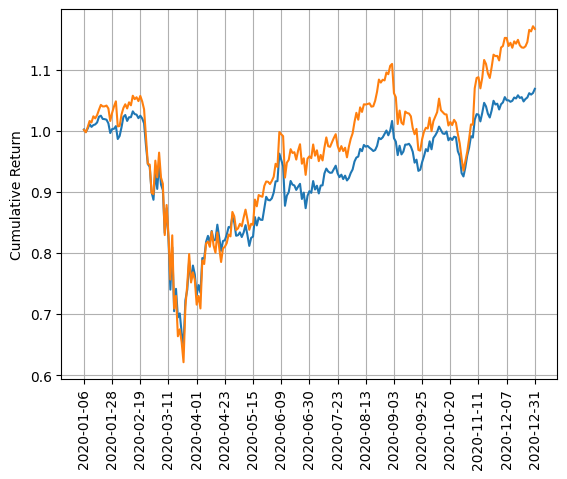
\includegraphics[width=0.6\linewidth]{figures/replica_portfolio}
%  \end{center}
%  \caption{Prob}
%  \label{fig:replica_portfolio_return}
%\end{figure}
%
%\begin{figure}[h]
%  \begin{center}
%    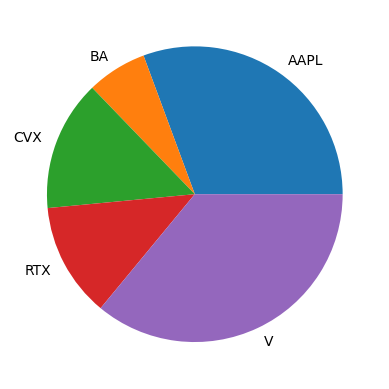
\includegraphics[width=0.6\linewidth]{figures/replica_portfolio_weights}
%  \end{center}
%  \caption{Prob}
%  \label{fig:replica_portfolio_weights}
%\end{figure}
%
%\begin{figure}[h]
%  \begin{center}
%    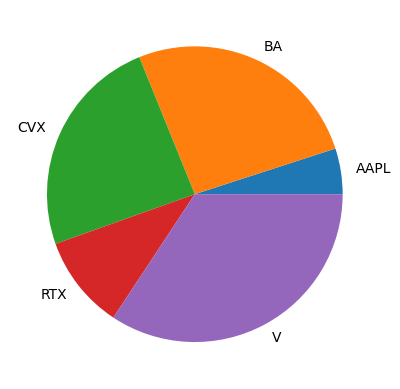
\includegraphics[width=0.6\linewidth]{figures/black_litterman_weights}
%  \end{center}
%  \caption{Prob}
%  \label{fig:black_litterman_weights}
%\end{figure}

\section{Risk Parity Portfolio}
\label{risk-parity-portfolio}

An alternative approach to optimize a portfolio is given by the \emph{risk parity}. A risk parity portfolio is an investment allocation strategy which focuses on the allocation of risk, rather than on the allocation of capital. 
Such a portfolio is characterized by having equal risk contributions to the total risk from each individual asset. 

This allocation strategy has gained popularity in the last decades since it is believed to provide better risk adjusted return than capital based allocation strategies.

Risk parity allocation is also referred to as equally-weighted risk contributions portfolio method. Equally-weighted risk contributions is not about \emph{having the same volatility}, it is about having each asset contributing in the same way to the portfolio overall volatility. For this we will have to define the contribution of each asset to the portfolio risk. 

Let's go over a very basic example to better illustrate how to construct a simple risk parity portfolio. Consider a portfolio of \(N\) assets: \(x_{1}, \ldots, x_N\) where as usual the weight of the $i^{th}$ asset is denoted by \(w_{i}\) and all the \(w_{i}\) form the allocation vector \(\mathbf{w}\). Let us further denote the covariance matrix of the assets as \(\Sigma\). The volatility of the portfolio is then defined as:

\begin{equation} 
\sigma_p={\sqrt {\mathbf{w}^T\Sigma \mathbf{w}}} = \sum_{i=1}^{N}\sigma _{i}\qquad\textrm{with}~\sigma _{i} = w_{i}\cdot \cfrac{\partial\sigma_p}{\partial w_{i}}={\cfrac {w_{i}(\Sigma \mathbf{w})_{i}}{\sqrt {\mathbf{w}^T\Sigma \mathbf{w}}}}
\end{equation}
so that \(\sigma _{i}\) can be interpreted as the contribution of the $i^{th}$ asset to the overall risk of the portfolio.

\begin{attention}
\subsubsection{Derivation of $\sigma_i$}
Expressing explicitly in matrix form the standard deviation of the portfolio we get
\[
\begin{split}
\sigma_p={\sqrt {\mathbf{w}^T\Sigma \mathbf{w}}} & =
\sqrt{
	\begin{bmatrix}
	w_{1} \\
	w_{2}
	\end{bmatrix}
	\begin{bmatrix}
	\sigma_{11} & \sigma_{21} \\
	\sigma_{12} & \sigma_{22} 
	\end{bmatrix}
	\begin{bmatrix}
	w_{1} & w_{2} \\
	\end{bmatrix}
}\\
&=
\sqrt{
	\begin{bmatrix}
	w_{1} \\
	w_{2}
	\end{bmatrix}
	\begin{bmatrix}
w_{1}\sigma_{11} + w_{2}\sigma_{12} & w_{1}\sigma_{21} + w_{2}\sigma_{22} \\
	\end{bmatrix}
} \\
&= \sqrt{
w_{1}w_{1}\sigma_{11} + w_{2}w_{1}\sigma_{12} + w_{1}w_{2}\sigma_{21} + w_{2}w_{2}\sigma_{22} }
\end{split}
\]
Now performing the derivative with respect to $w_1$ we obtain
\[\cfrac{\partial\sigma_p}{\partial w_1} = \cfrac{1}{2}\cdot\cfrac{2\cdot w_1\sigma_{11} + 2\cdot w_{2}\sigma_{21}}{\sigma_p} = \cfrac{w_1\sigma_{11} + w_{2}\sigma_{21}}{\sigma_p} = \cfrac{(\Sigma \mathbf{w})_{1}}{\sigma_p}\]
	
Summing up $\sum_{i=1}^{N} w_i\cdot\cfrac{\partial\sigma_p}{\partial w_i}$ we get back $\sigma_p$
\end{attention}

Equal risk contribution then means \(\sigma _{i} =\sigma _{j}\) for all \(i,j\) or equivalently \(\sigma _{i}=\sigma_p/N\). So

\begin{equation}
\sigma _{i} = \cfrac{\sigma_p}{N}={\cfrac {w_{i}(\Sigma \mathbf{w})_{i}}{\sqrt {\mathbf{w}^T\Sigma \mathbf{w}}}}\implies w_{i} = \frac {\sigma_p^{2}}{(\Sigma \mathbf{w})_{i}N}
\label{eq:risk_parity_weights}
\end{equation}
Since we want the previous expression to be true for each $i$, the solution for the weights can be found by solving the minimization problem

\begin{equation} 
\underset{\mathbf{w}}{\min } \sum _{i=1}^{N}\left[w_{i}-{\frac {\sigma_p^{2}}{(\Sigma \mathbf{w})_{i}N}}\right]^{2} 
\end{equation}
\noindent
where ideally it is required to be 0 the difference between the squared sum of the weights and the theoretical values expressed by Eq~\ref{eq:risk_parity_weights}.

Going back to our data sample let's find out the weights to give us a risk parity portfolio.

\begin{ipython}
num_assets = 5
def risk_parity(w, cov):
    variance = w.T.dot(cov.dot(w))
    *@sum@* = 0
    N = len(w)
    for i in range(N):
        *@sum@* += (w[i] - (variance/(N*cov.dot(w)[i])))**2
    return *@sum@*
	
args = (covariance,)
constraints = ({'type': 'eq', 'fun': sum_weights})
bounds = tuple((0, 1) for asset in range(num_assets))
weights = [1./num_assets for _ in range(num_assets)]
opts = minimize(risk_parity, weights, args=(covariance,),
                bounds=bounds, constraints=constraints)
print (opts)
\end{ipython}
\begin{ioutput}
    fun: 2.2881862766486147e-07
    jac: array([-6.98851511e-04,  1.92391042e-04, -4.08403758e-05, 
                -2.54432521e-05,  1.13250609e-03])
message: 'Optimization terminated successfully.'
   nfev: 38
    nit: 5
   njev: 5
 status: 0
success: True
x: array([0.25863039, 0.18154282, 0.19666705, 0.22190633, 
          0.14125342])
\end{ioutput}

\begin{ipython}
sigma_i = []
std = np.sqrt(opts.x.T.dot(covariance.dot(opts.x)))
for i in range(num_assets):
    a = opts.x[i]*covariance.dot(opts.x)[i]
	sigma_i.append(a/std)
	
for i in range(num_assets):
    print (f"Risk contribution for asset {i}: {sigma_i[i]/sum(sigma_i)*100:.3f}%")
\end{ipython}
\begin{ioutput}
Risk contribution for asset 0: 19.974%
Risk contribution for asset 1: 19.999%
Risk contribution for asset 2: 19.990%
Risk contribution for asset 3: 19.992%
Risk contribution for asset 4: 20.045%
\end{ioutput}

Figure~\ref{fig:risk_parity} shows the fraction of risk allocated to each asset with the corresponding weight within the portfolio.

\begin{figure}[htb]
\centering
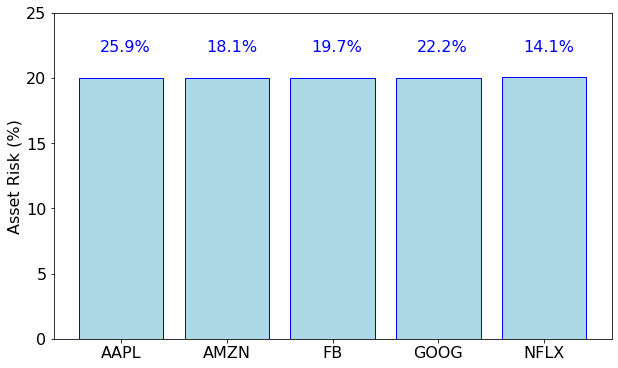
\includegraphics[width=0.7\textwidth]{figures/risk_parity}
\caption{Fraction of risk allocated among the assets of a portfolio. The blue numbers show the corresponding weight of each asset.}
\label{fig:risk_parity}
\end{figure}

\subsection{Risk Budget Allocation}
\label{risk-budget-allocation}

The same technique can be used if we would like to calculate a portfolio with risk budget allocation. In this case we want to associate to each asset a particular level of risk.We can now change the previous equation which was setting every asset risk contribution fraction to $1/N$

\begin{equation} 
\sigma _{i}=\cfrac{\sigma_p}{N} 
\end{equation}
and replace it with the desired fraction of risk (\(f_i\)) specific for each asset

\begin{equation} 
\sigma _{i}=f_i \cdot \sigma_p 
\end{equation}
so that the relation to minimize becomes

\begin{equation} 
\underset{\mathbf{w}}{\min} \sum _{i=1}^{N}\left[w_{i}-{\frac {f_i \cdot \sigma_p^{2}}{(\Sigma \mathbf{w})_{i}}}\right]^{2} 
\end{equation}
\noindent
Translating it into \texttt{python} we get:
\begin{ipython}
def risk_budget(w, target_risk, cov):
    variance = w.T.dot(cov.dot(w))
    *@sum@* = 0
    N = len(w)
    for i in range(N):
        *@sum@* += (w[i] - (target_risk[i]*variance)/(cov.dot(w)[i]))**2
    return *@sum@*
	
f_i = [0.3, 0.2, 0.2, 0.15, 0.15]
args = (f_i, covariance)
constraints = ({'type': 'eq', 'fun': sum_weights})
bounds = tuple((0, 1) for asset in range(num_assets))
weights = [1./num_assets for _ in range(num_assets)]
opts = minimize(risk_budget, weights, args=(f_i, covariance),
                bounds=bounds, constraints=constraints)
print (opts)
\end{ipython}
\begin{ioutput}
    fun: 4.058673684147486e-08
    jac: array([-2.64817707e-04,  3.30937403e-04,  2.14530647e-05, 
                -7.65372775e-05,  3.67853561e-04])
message: 'Optimization terminated successfully.'
   nfev: 45
    nit: 6
   njev: 6
 status: 0
success: True
      x: array([0.3459366 , 0.1800917 , 0.19394454, 0.16890483, 
                0.11112233])
\end{ioutput}
\begin{ipython}  
sigma_i = []
std = np.sqrt(opts.x.T.dot(covariance.dot(opts.x)))
for i in range(num_assets):
    a = opts.x[i]*covariance.dot(opts.x)[i]
    sigma_i.append(a/std)
	
for i in range(num_assets):
    print (f"Risk contribution for asset {i}: {sigma_i[i]/sum(sigma_i)*100:.3f}%")    
\end{ipython}
\begin{ioutput}
Risk contribution for asset 0: 29.988%
Risk contribution for asset 1: 20.010%
Risk contribution for asset 2: 19.996%
Risk contribution for asset 3: 14.993%
Risk contribution for asset 4: 15.012%
\end{ioutput}

Figure~\ref{fig:risk_allocation} shows the amount of risk associated to each asset and its weight within the portfolio. 
Indeed for each stock we have allocated the desired amount of risk.

\begin{figure}[htb]
\centering
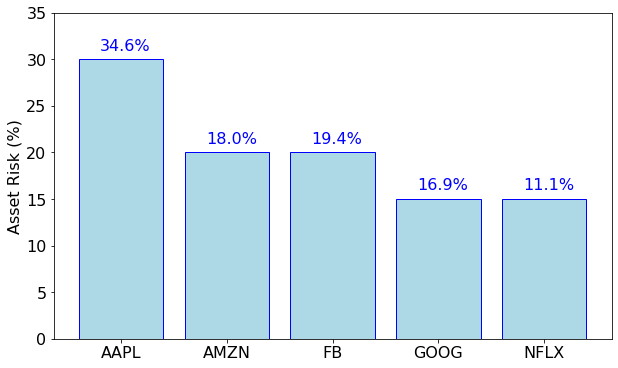
\includegraphics[width=0.7\textwidth]{figures/risk_allocation}
\caption{Fraction of risk allocated among the assets of a portfolio. The blue numbers show the corresponding weight of each asset.}
\label{fig:risk_allocation}
\end{figure}

%\subsection{Maximum Diversification Portfolio}
%\label{maximum-diversification-portfolio}
%
%Diversification is most often either pursued in tandem with other objective, such as return maximization, or pursued simply by including more asset classes or adding constraints based on intuition.
%
%But it does not have to be this way and diversification can be pursued explicitly as the sole objective in portfolio construction.
%In a 2008 paper~\cite{bib:diversification}, the diversification ratio $D$ of a portfolio has been defined as
%
%\begin{equation}
%D=\cfrac{\mathbf{w}^T\boldsymbol{\sigma}}{\sqrt {\mathbf{w}^T\Sigma \mathbf{w}}} 
%\end{equation}
%where $\boldsymbol{\sigma}$ is the vector of volatilities and $\Sigma$ is the covariance matrix. The denominator represents portfolio volatility and the numerator the asset weighted average volatilities. More diversification within a portfolio decreases the denominator and leads to a higher diversification ratio.
%Let's construct a portfolio that maximize this ratio.
%
%\begin{ipython}
%def diversification_ratio(w):
%    w_vol = np.dot(np.sqrt(np.diag(covariance)), w.T)
%    port_vol = np.sqrt(np.dot(w.T, np.dot(covariance, w)))
%    diversification_ratio = w_vol/port_vol
%    return -diversification_ratio
%	
%bounds = tuple((0, 1) for asset in range(num_assets))
%cons = ({'type': 'eq', 'fun': sum_weights},)
%#cons = cons + ({'type': 'ineq', 'fun': long_only_constraint},)
%weights = [1./num_assets for _ in range(num_assets)]
%opts = minimize(diversification_ratio, weights, bounds=bounds,
%                constraints=cons)
%print (opts)
%\end{ipython}
%\begin{ioutput}
%    fun: -1.3580745811820554
%    jac: array([-0.00035974,  0.00029349, -0.00035594,  0.00077944,  
%                 0.00016446])
%message: 'Optimization terminated successfully.'
%   nfev: 36
%    nit: 5
%   njev: 5
% status: 0
%success: True
%      x: array([0.34867985, 0.18062199, 0.15557008, 0.1235694, 0.19155868])
%\end{ioutput}
%\begin{ipython}
%ret = np.sum(returns*opts.x)
%vol = np.sqrt(opts.x.T.dot(np.dot(covariance, opts.x))) 
%print ("Return: ", ret)
%print ("Vol: ", vol)
%print ("Diversification: ", -opts.fun)
%\end{ipython}
%\begin{ioutput}
%Return:  0.32143376694380044
%Vol:  0.20743461253140413
%Diversification:  1.360393553158368
%\end{ioutput}
%
%Figure~\ref{fig:max_div} shows how the maximum diversified portfolio compares to the efficient frontier.
%
%\begin{figure}[htb]
%\centering
%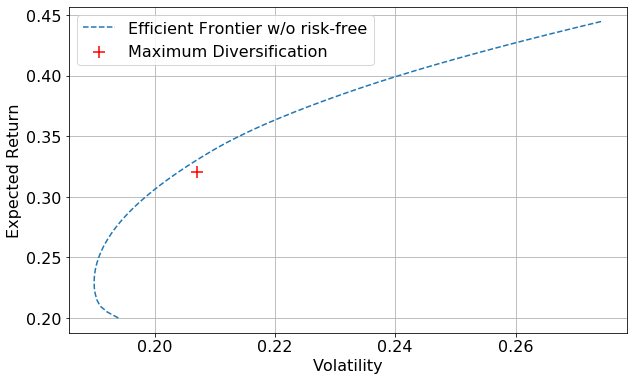
\includegraphics[width=0.7\textwidth]{figures/max_div}
%\caption{Portfolio constructed with the maximum diversification technique shown in the return/variance plane.}
%\label{fig:max_div}
%\end{figure}

\section*{Exercises}
\begin{question}
One of the approaches to finding the optimal point on the efficient frontier for a given investor is to maximize the investor's utility ($U$). This is a measure of how much benefit investors obtain from portfolio performance. Utility is a measure of relative satisfaction that an investor derives from different portfolios. Utility is a function of the portfolio expected return, the portfolio variance and a measure of risk aversion

\begin{equation*}
U = \mathbb{E}(R_{p}) - \frac{1}{2}A\sigma^2
\end{equation*}
where $U$ = utility, $\mathbb{E}(R)$ = portfolio expected return, $A$ = risk aversion coefficient and $\sigma^2$ = portfolio variance.
In determining the risk aversion ($A$), we measure the marginal reward an investor needs in order to take on more risk. A risk-averse investor will need a high margin reward for taking on more risk. The utility equation shows the following:
\begin{itemize}
\tightlist
\item $U$ can be positive or negative, i.e. it is unbounded;
\item high returns add to utility;
\item high variance reduces utility;
\item $U$ does not measure satisfaction but can be used to rank portfolios.
\end{itemize}

The risk aversion coefficient, $A$, ranges between 1 and 10 (1 for the aggressive investor, 4 for the moderate investor, and 10 for the risk-averse investor.

Given the historical series in \href{https://github.com/matteosan1/finance_course/raw/master/input_files/share_price.csv}{share\_prices.csv} find the best portfolio for aggressive, moderate and risk-averse investors.

\end{question}

\cprotEnv \begin{solution}
\begin{ipython}
import pandas as pd
df = pd.read_csv("share_prices.csv", index_col='Date')
daily_returns = df.pct_change()
returns = daily_returns.mean()*252
covariance = daily_returns.cov()*252

print (returns)
print (covariance)
\end{ipython}
\begin{ioutput}
CHD     0.062666
COST    0.247429
CTRE    0.165151
ENTR    0.002445
HI      0.223906
LDOS    0.075464
TDS    -0.003953
TMUS    0.283815
UEC     0.999521
WM      0.163298
dtype: float64

           CHD     COST       CTRE      ENTR        HI      LDOS       TDS
CHD   0.067815  0.036114  0.016454  0.022583  0.022301  0.029738  0.032921   
COST  0.036114  0.073004  0.031599  0.049279  0.034606  0.034481  0.034043   
CTRE  0.016454  0.031599  0.313706  0.074262  0.136719  0.068927  0.088424   
ENTR  0.022583  0.049279  0.074262  0.113892  0.062266  0.043155  0.040843   
HI    0.022301  0.034606  0.136719  0.062266  0.202751  0.068284  0.097420   
LDOS  0.029738  0.034481  0.068927  0.043155  0.068284  0.110635  0.059296   
TDS   0.032921  0.034043  0.088424  0.040843  0.097420  0.059296  0.185842   
TMUS  0.026069  0.042121  0.073199  0.055806  0.057519  0.046704  0.068516   
UEC   0.045100  0.099269  0.164647  0.147985  0.165341  0.096700  0.143037   
WM    0.034987  0.034676  0.049294  0.034555  0.057760  0.047310  0.048338   
...
\end{ioutput}
\begin{ipython}
import numpy as np
from scipy.optimize import minimize

def sum_weights(w): 
    return np.sum(w) - 1

def utility(w, returns, cov, risk_aversion):
    return -(returns.dot(w) - 0.5*w.T.dot(cov.dot(w))*risk_aversion)

num_assets = 10
constraints = [{'type': 'eq', 'fun': sum_weights},] 
bounds = tuple((0, 1) for _ in range(num_assets))
weights = [1./num_assets for _ in range(num_assets)]

for risk_aversion in (1, 4, 10):
  opts = minimize(utility, weights, args=(returns, covariance, risk_aversion),
                bounds=bounds, constraints=constraints)
  for i, c in enumerate(df.columns):
    print ("{} {:.1f}".format(c, opts.x[i]*100), end=" ")
  print()
  print ("Expected return: {:.3f}".format(opts.x.dot(returns)))
  print ("Variance: {:.3f}".format(opts.x.T.dot(covariance.dot(opts.x))))
\end{ipython}
\begin{ioutput}
# aggressive
CHD 0.0 COST 0.0 CTRE 0.0 ENTR 0.0 HI 0.0 LDOS 0.0 TDS 0.0 TMUS 12.8 UEC 87.2 WM 0.0 
Expected return: 0.908
Variance: 0.734

# moderate
CHD 0.0 COST 47.2 CTRE 0.0 ENTR 0.0 HI 0.0 LDOS 0.0 TDS 0.0 TMUS 33.1 UEC 18.3 WM 1.4 
Expected return: 0.396
Variance: 0.104

# risk averse
CHD 7.1 COST 40.2 CTRE 0.0 ENTR 0.0 HI 1.3 LDOS 0.0 TDS 0.0 TMUS 22.7 UEC 4.1 WM 24.6 
Expected return: 0.252
Variance: 0.055
\end{ioutput}
\end{solution}

\begin{question}
Your are portfolio manager and one of your clients is asking to design her investment in order to reduce at the minimum the risk. Her position involves these shares: 'TMUS', 'TDS', 'ENTR', 'UEC', 'WM', 'CTRE', 'LDOS', 'COST', 'CHD', 'HI'.
Find the weights corresponding to each asset.

\noindent\textbf{Hint:} the historical series of the corresponding companies are stored in \href{https://github.com/matteosan1/finance_course/raw/master/input_files/share_price.csv}{share\_prices.csv}.

\end{question}

\cprotEnv \begin{solution}
\begin{ipython}
import pandas as pd
df = pd.read_csv("share_prices.csv", index_col='Date')

daily_returns = df.pct_change()
returns = daily_returns.mean()*252
covariance = daily_returns.cov()*252
\end{ipython}
\begin{ipython}
import numpy as np
from scipy.optimize import minimize

def sum_weights(w):
    return np.sum(w) - 1

def min_risk(w, cov):
    return np.sqrt(w.T.dot(cov.dot(w)))

num_assets = 10
constraints = ({'type': 'eq', 'fun': sum_weights},)
bounds = tuple((0, 1) for asset in range(num_assets))
weights = [1./num_assets for _ in range(num_assets)]
opts = minimize(min_risk, weights, args=(covariance,),
                bounds=bounds, constraints=constraints)

print (opts)
\end{ipython}
\begin{ioutput}
     fun: 0.20887087318996655
     jac: array([0.2088003 , 0.20897953, 0.20895358, 0.20911743, 0.21106115,
                 0.20858843, 0.20914311, 0.20901022, 0.40519709, 0.20881298])
 message: 'Optimization terminated successfully'
    nfev: 110
     nit: 10
    njev: 10
  status: 0
 success: True
       x: array([3.33744344e-01, 1.68530140e-01, 8.18977235e-03, 9.91808728e-02,
                 0.00000000e+00, 7.10377889e-02, 6.05724516e-03, 8.44657341e-02,
                 3.89635156e-20, 2.28794102e-01])
\end{ioutput}
\begin{ipython}
print ("Portfolio composition")
for i, n in enumerate(df.columns):
    print ("{:5}: {:4.1f}%".format(n, opts.x[i]*100))
print ("Portfolio variance: {:.4f}".format(opts.fun**2))
print ("Expected Portfolio return: {:.3f}".format(opts.x.dot(returns)))
\end{ipython}
\begin{ioutput}
Portfolio composition
CHD  : 33.4%
COST : 16.9%
CTRE :  0.8%
ENTR :  9.9%
HI   :  0.0%
LDOS :  7.1%
TDS  :  0.6%
TMUS :  8.4%
UEC  :  0.0%
WM   : 22.9%
Portfolio variance: 0.0436
Expected Portfolio return: 0.131
\end{ioutput}
\end{solution}

%\begin{question}[title={(Return Allocation Portfolio)}]
%After few months the same client of the previous question, contacted you again asking for larger returns. In particular she would like to increase it by 40\%.
%Find the new portfolio composition that makes your client happy.
%\end{question}
%\begin{solution}
%\begin{tcolorbox}[size=fbox, boxrule=1pt, colback=cellbackground, colframe=cellborder]
%\begin{Verbatim}[commandchars=\\\{\}]
%\PY{k}{def} \PY{n+nf}{efficient\PYZus{}frontier}\PY{p}{(}\PY{n}{w}\PY{p}{,} \PY{n}{asset\PYZus{}returns}\PY{p}{,} \PY{n}{target\PYZus{}return}\PY{p}{)}\PY{p}{:} 
%    \PY{n}{portfolio\PYZus{}return} \PY{o}{=} \PY{n}{np}\PY{o}{.}\PY{n}{sum}\PY{p}{(}\PY{n}{asset\PYZus{}returns} \PY{o}{*} \PY{n}{w}\PY{p}{)} 
%    \PY{k}{return} \PY{p}{(}\PY{n}{portfolio\PYZus{}return} \PY{o}{\PYZhy{}} \PY{n}{target\PYZus{}return}\PY{p}{)}
%		
%\PY{n}{results} \PY{o}{=} \PY{p}{[}\PY{p}{]}
%\PY{n}{bounds} \PY{o}{=} \PY{n+nb}{tuple}\PY{p}{(}\PY{p}{(}\PY{l+m+mi}{0}\PY{p}{,} \PY{l+m+mi}{1}\PY{p}{)} \PY{k}{for} \PY{n}{asset} \PY{o+ow}{in} \PY{n+nb}{range}\PY{p}{(}\PY{n}{num\PYZus{}assets}\PY{p}{)}\PY{p}{)}
%\PY{n}{target} \PY{o}{=} \PY{l+m+mf}{0.172}\PY{o}{*}\PY{l+m+mf}{1.4}
%\PY{n}{constraints} \PY{o}{=} \PY{p}{(}\PY{p}{\PYZob{}}\PY{l+s+s1}{\PYZsq{}}\PY{l+s+s1}{type}\PY{l+s+s1}{\PYZsq{}}\PY{p}{:} \PY{l+s+s1}{\PYZsq{}}\PY{l+s+s1}{eq}\PY{l+s+s1}{\PYZsq{}}\PY{p}{,} \PY{l+s+s1}{\PYZsq{}}\PY{l+s+s1}{fun}\PY{l+s+s1}{\PYZsq{}}\PY{p}{:} \PY{n}{efficient\PYZus{}frontier}\PY{p}{,} 
%                \PY{l+s+s1}{\PYZsq{}}\PY{l+s+s1}{args}\PY{l+s+s1}{\PYZsq{}}\PY{p}{:}\PY{p}{(}\PY{n}{returns}\PY{p}{,} \PY{n}{target}\PY{p}{)}\PY{p}{\PYZcb{}}\PY{p}{,}
%               \PY{p}{\PYZob{}}\PY{l+s+s1}{\PYZsq{}}\PY{l+s+s1}{type}\PY{l+s+s1}{\PYZsq{}}\PY{p}{:} \PY{l+s+s1}{\PYZsq{}}\PY{l+s+s1}{eq}\PY{l+s+s1}{\PYZsq{}}\PY{p}{,} \PY{l+s+s1}{\PYZsq{}}\PY{l+s+s1}{fun}\PY{l+s+s1}{\PYZsq{}}\PY{p}{:} \PY{n}{sum\PYZus{}weights}\PY{p}{\PYZcb{}}\PY{p}{)}
%\PY{n}{weights} \PY{o}{=} \PY{p}{[}\PY{l+m+mf}{1.}\PY{o}{/}\PY{n}{num\PYZus{}assets} \PY{k}{for} \PY{n}{\PYZus{}} \PY{o+ow}{in} \PY{n+nb}{range}\PY{p}{(}\PY{n}{num\PYZus{}assets}\PY{p}{)}\PY{p}{]}
%\PY{n}{opts} \PY{o}{=} \PY{n}{minimize}\PY{p}{(}\PY{n}{markowitz}\PY{p}{,} \PY{n}{weights}\PY{p}{,} \PY{n}{args}\PY{o}{=}\PY{p}{(}\PY{n}{covariance}\PY{p}{,}\PY{p}{)}\PY{p}{,}
%\PY{n}{bounds}\PY{o}{=}\PY{n}{bounds}\PY{p}{,} \PY{n}{constraints}\PY{o}{=}\PY{n}{constraints}\PY{p}{)} 
%		
%\PY{n}{p\PYZus{}variance} \PY{o}{=} \PY{n}{np}\PY{o}{.}\PY{n}{dot}\PY{p}{(}\PY{n}{opts}\PY{o}{.}\PY{n}{x}\PY{o}{.}\PY{n}{T}\PY{p}{,} \PY{n}{np}\PY{o}{.}\PY{n}{dot}\PY{p}{(}\PY{n}{covariance}\PY{p}{,} \PY{n}{opts}\PY{o}{.}\PY{n}{x}\PY{p}{)}\PY{p}{)}
%\PY{n}{ret} \PY{o}{=} \PY{n}{np}\PY{o}{.}\PY{n}{sum}\PY{p}{(}\PY{n}{returns}\PY{o}{*}\PY{n}{opts}\PY{o}{.}\PY{n}{x}\PY{p}{)}
%\PY{n+nb}{print} \PY{p}{(}\PY{l+s+s2}{\PYZdq{}}\PY{l+s+s2}{Portfolio variance: }\PY{l+s+si}{\PYZob{}:.3f\PYZcb{}}\PY{l+s+s2}{\PYZdq{}}\PY{o}{.}\PY{n}{format}\PY{p}{(}\PY{n}{variance}\PY{p}{)}\PY{p}{)}
%\PY{n+nb}{print} \PY{p}{(}\PY{l+s+s2}{\PYZdq{}}\PY{l+s+s2}{Portfolio return: }\PY{l+s+si}{\PYZob{}:.3f\PYZcb{}}\PY{l+s+s2}{\PYZdq{}}\PY{o}{.}\PY{n}{format}\PY{p}{(}\PY{n}{ret}\PY{p}{)}\PY{p}{)}
%
%Portfolio variance: 0.026
%Portfolio return: 0.241
%\end{Verbatim}
%\end{tcolorbox}	
%\end{solution}

\begin{question}
The client is not yet satisfied and decides to move to a risk parity portfolio. Compute the correct weights to have each asset contributing equally to the portfolio risk.
\end{question}

\cprotEnv \begin{solution}
\begin{ipython}
def risk_parity(w, cov):
    variance = w.T.dot(cov.dot(w))
    sum = 0 
    N = len(w)
    for i in range(N):
        sum += (w[i] - (variance/(N*(cov.dot(w))[i])))**2
    return sum

args = (covariance,)
constraints = ({'type': 'eq', 'fun': sum_weights})
bounds = tuple((0, 1) for asset in range(num_assets))
weights = [1./num_assets for _ in range(num_assets)]
opts = minimize(risk_parity, weights, args=(covariance,),
                bounds=bounds, constraints=constraints)

print (opts)
\end{ipython}
\begin{ioutput}
     fun: 3.5766519241779855e-07
     jac: array([ 1.24834913e-03,  1.00388202e-03, -2.28052647e-04,  6.19051279e-04,
                 -5.68149005e-04, -1.03169022e-03, -1.24285291e-03, -4.09550915e-04,
                 -2.02491654e-03,  6.26250036e-06])
 message: 'Optimization terminated successfully'
    nfev: 80
     nit: 7
    njev: 7
  status: 0
 success: True
       x: array([0.161952  , 0.12997992, 0.07022277, 0.10331577, 0.07717795,
                 0.10490077, 0.08475445, 0.10276264, 0.04079525, 0.12413849])
\end{ioutput}
\begin{ipython}
sigma_i = []
for i in range(num_assets):
    std = np.sqrt(opts.x.T.dot(covariance.dot(opts.x)))
    a = opts.x[i]*covariance.dot(opts.x)[i]
    sigma_i.append(a/std)

for i in range(num_assets):
    print ("Risk contribution for asset {}: {:6.3f}%"
           .format(i, sigma_i[i]/sum(sigma_i)*100))
\end{ipython}
\begin{ioutput}
Risk contribution for asset 0:  9.986%
Risk contribution for asset 1: 10.003%
Risk contribution for asset 2:  9.971%
Risk contribution for asset 3:  9.987%
Risk contribution for asset 4: 10.014%
Risk contribution for asset 5:  9.998%
Risk contribution for asset 6: 10.047%
Risk contribution for asset 7:  9.976%
Risk contribution for asset 8: 10.023%
Risk contribution for asset 9:  9.995%		
\end{ioutput}
\end{solution}



\begin{thebibliography}{9}
\bibitem{bib:post_modern_theory}\href{https://en.wikipedia.org/wiki/Post-modern_portfolio_theory}{\emph{Post Modern Theory}}, Wikipedia [Online]
%\bibitem{bib:black_litterman}\href{https://en.wikipedia.org/wiki/Black\%E2\%80\%93Litterman_model}{\emph{Black-Litterman Model}}, Wikipedia [Online]
\bibitem{bib:bl_prior} F. Black, R. Litterman, \emph{Combining investor views with market equilibrium.}, The Journal of Fixed Income, 1991.
\bibitem{bib:Idzorek} T. Idzorek, \emph{A step-by-step guide to the Black-Litterman model: Incorporating user-specified confidence levels.}, Elsevier Ltd; 2007. p. 17–38.
\bibitem{bib:tau} J. Walters, \href{https://ssrn.com/abstract=1701467}{\emph{The Factor Tau in the Black-Litterman Model}}, October 9, 2013
\bibitem{bib:walters} J. Walters, \emph{The Black-Litterman Model in Detail}, SSRN Electron J.;(February 2007):1–65
\bibitem{bib:diversification} Y. Choueifaty, Y.Coignard, \href{ https://www.tobam.fr/wp-content/uploads/2014/12/TOBAM-JoPM-Maximum-Div-2008.pdf}{\emph{Toward Maximum Diversification}}, 2008
\end{thebibliography}
